\documentclass[aspectratio=169]{beamer}
% ============================================================================
% HEC Montréal MBA -- ECON50803: Environnement macroéconomique
% Shared Beamer Preamble
% ============================================================================
% Loads jfb-teaching-slides.sty from latex-common (sibling repo) for the full
% teaching Beamer aesthetic: Fira Sans fonts, HEC palette, titleframe /
% sectionframe, box envs (keyinsight, bizimplication, warning, defbox,
% exercise), newspaper headlines, backup slides, TikZ styles for AD-AS and
% supply/demand diagrams.
%
% Course-specific configuration, project paths, and overrides live below.
% ============================================================================

\usepackage{jfb-teaching-slides}

% --- Course metadata (drives the footer) ------------------------------------
\jfbcoursename{ECON 50803}
\jfbcoursetitle{Environnement macroéconomique}
\jfbinstitution{HEC Montréal}

% --- Project paths ----------------------------------------------------------
\graphicspath{{../Figures/}}
\newcommand*\includetables[1]{\input{../Tables/#1.tex}}

% --- Shared closing roadmap -----------------------------------------------
% The argument is the session just completed. On the white slide background,
% HECnavy!40 gives completed themes the appearance of 40% opacity.
\newcommand{\coursethemestyle}[3]{%
   \ifnum#1>#2\relax
      \textcolor{HECnavy}{#3}%
   \else
      \textcolor{HECnavy!40}{#3}%
   \fi
}
\newcommand{\courseroadmap}[1]{%
   \begin{frame}{Les thèmes du cours}
      \renewcommand{\arraystretch}{1.4}
      \centering
      \small
      \begin{tabularx}{\textwidth}{>{\bfseries\raggedright\arraybackslash}X >{\raggedright\arraybackslash}p{0.40\textwidth}}
         \toprule
         \textbf{Question centrale} & \textbf{Séance} \\
         \midrule
         \coursethemestyle{1}{#1}{Comment mesurer la production, les prix et le niveau de vie\,?} & \coursethemestyle{1}{#1}{S1 : Mesurer l'économie} \\
         \coursethemestyle{2}{#1}{Pourquoi certains pays sont-ils plus riches que d'autres\,?} & \coursethemestyle{2}{#1}{S2 : Croissance de long terme} \\
         \coursethemestyle{3}{#1}{Qu'est-ce qui détermine l'emploi, les salaires et l'investissement\,?} & \coursethemestyle{3}{#1}{S3 : Marchés du travail et du capital} \\
         \coursethemestyle{4}{#1}{Pourquoi l'économie connaît-elle des hauts et des bas\,?} & \coursethemestyle{4}{#1}{S4 : Cycles économiques} \\
         \coursethemestyle{5}{#1}{Pourquoi et comment combattre les récessions\,?} & \coursethemestyle{5}{#1}{S5 : Politique monétaire et budgétaire} \\
         \bottomrule
      \end{tabularx}
   \end{frame}
}

% --- TikZ style overrides (preserve pre-migration visual choices) ----------
% The shared jfb-teaching-slides.sty defines stronger defaults (e.g.
% supply/demand in HECnavy, eqpoint default HECgreen). Keep the original
% ECON50803 overrides here so existing slides render unchanged.
\tikzset{
   supply/.style     = {very thick},
   original/.style   = {HECgray, thick, dashed},
   refline/.style    = {thin, dashed, HECgray},
   shiftarrow/.style = {very thick, -Stealth},
   eqpoint/.default  = HECnavy,
   eqfaded/.style    = {fill=HECgray, draw=HECgray, opacity=0.4},
   potline/.style    = {HECgreen, thick, dashed},
   econbrace/.style  = {decorate, decoration={brace, amplitude=6pt, mirror}, thick},
   pointlabel/.style = {font=\small},
   annotlabel/.style = {font=\small},
}

% --- Exam-relevance tag -----------------------------------------------------
% Set \showexamtagstrue and rebuild all sessions before the exam.
\newif\ifshowexamtags
\showexamtagsfalse
\usetikzlibrary{shapes.geometric}
\newcommand{\examtag}{%
   \ifshowexamtags%
      \begin{tikzpicture}[remember picture, overlay]
         \node[star, star points=5, star point ratio=2.25,
               fill=HECcoral, inner sep=1.6pt, anchor=north east]
            at ([xshift=-0.5cm, yshift=-0.65cm]current page.north east) {};
      \end{tikzpicture}%
   \fi%
}

\graphicspath{{../Figures/}}
\jfbcoursename{L'essentiel du MBA}
\jfbcoursetitle{Environnement macroéconomique}
\title{Environnement macroéconomique}
\author{Jean-Félix Brouillette}
\date{L'essentiel du MBA\\École des dirigeants\\Édition octobre 2026}

% Build from Slides/ESS_MBA/: latexmk -pdf ess_mba.tex
% 78 static slides: 70 selected S1--S5 frames, a shared title frame,
% four shared section frames, a resource guide and two closing summaries.
% ECON50803 visual identity is inherited from preamble.tex without overrides.
% Figures remain shared vector assets with their original source vintages.
% Only standalone-course references, minor accuracy/clarity points and
% necessary layout/arrow repairs are adapted in the copied frames.
% Source provenance and any adaptation appear above each selected frame.
% Timing, including a 10-minute break after slide 47: 3h30.
\newcolumntype{J}{>{\raggedright\arraybackslash}X}
\begin{document}

% ============================================================================
% 01 | \titleframe
% Source: Shared ECON50803 title/section style
% ============================================================================
\titleframe

% ============================================================================
% 02 | \begin{frame}{Un monde complexe et incertain}
% Source: S1/s1.tex | \begin{frame}{Un monde complexe et incertain}
% ============================================================================
\begin{frame}{Un monde complexe et incertain}
   \begin{tikzpicture}[remember picture, overlay]
      \setcounter{newshl}{0}
      % The Globe and Mail, 2026-09-15; headline supplied by the user.
      \newsheadline[globeandmail]{The Globe and Mail}{\href{https://www.theglobeandmail.com/business/article-carney-tax-mega-deduction-investment-summit/}{\guillemotleft~Ottawa plans `mega deduction' tax incentive to spur investment~\guillemotright}}
      % Financial Times, 2026-08-26; verified in the publisher's search results on 2026-10-15.
      \newsheadline[ft]{Financial Times}{\href{https://www.ft.com/content/9cb63980-cd43-419d-a7e5-42039b9fd01e?syn-25a6b1a6=1}{\guillemotleft~The multiplying risks of financing data centres~\guillemotright}}
      % Bloomberg, 2026-09-23.
      \newsheadline[bloomberg]{Bloomberg}{\href{https://www.bloomberg.com/news/articles/2026-09-23/us-treasury-five-year-yields-breach-5-for-first-time-since-2007}{\guillemotleft~US Bond-Market Slide Deepens, Pushing Yields to Two-Decade Highs~\guillemotright}}
      % Reuters, 2026-10-07; syndicated by The Edge Malaysia.
      \newsheadline[reuters]{Reuters}{\href{https://theedgemalaysia.com/node/820812}{\guillemotleft~Oil rises as investors weigh supply threats~\guillemotright}}
      % La Presse, 2026-10-06; verified in the publisher's page metadata on 2026-10-15.
      % Section kicker omitted: Étude de la Banque du Canada.
      \newsheadline[lapresse]{La Presse}{\href{https://www.lapresse.ca/affaires/economie/2026-10-06/etude-de-la-banque-du-canada/la-replique-tarifaire-du-canada-alimente-l-inflation.php}{\guillemotleft~La réplique tarifaire du Canada alimente l'inflation~\guillemotright}}
      % Le Devoir, 2026-10-09; current title and canonical URL verified on the publisher's page on 2026-10-15.
      \newsheadline[ledevoir]{Le Devoir}{\href{https://www.ledevoir.com/economie/1015754/economie-quebecoise-perdu-49-000-emplois-septembre}{\guillemotleft~L'économie québécoise a perdu 49\,000 emplois en septembre~\guillemotright}}
% Static summary: retain the original headline slide without its second overlay.
   \end{tikzpicture}
\end{frame}

% ============================================================================
% 03 | \begin{frame}[t]{Pourquoi la macroéconomie \textit{vous} concerne-t-elle\,?}
% Source: S1/s1.tex | \begin{frame}[t]{Pourquoi la macroéconomie \textit{vous} concerne-t-elle\,?}
% ============================================================================
\begin{frame}[t]{Pourquoi la macroéconomie \textit{vous} concerne-t-elle\,?}
   \small\raggedright
   Les événements macroéconomiques perturbent les \textbf{stratégies d'affaires}, influencent les \textbf{coûts, salaires et taux d'intérêt}, et sont sources de \textbf{risque} mais aussi d'\textbf{opportunité}. \\ \vspace{0.25cm}

   Les entreprises dont les gestionnaires font de \textbf{meilleures prévisions macroéconomiques} sont plus \textbf{productives}, plus \textbf{rentables} et captent une plus grande \textbf{part de marché}.
   \vspace{0.1cm}
   \begin{itemize}
      \footnotesize
      \setlength\itemsep{0.1cm}
      \item[\textcolor{HECgray}{$\bullet$}] {\color{HECgray} Tanaka, Bloom, David \& Koga, \textit{J.\ Monetary Econ.}, 2020}
      \item[\textcolor{HECgray}{$\bullet$}] {\color{HECgray} Bloom, Kawakubo, Meng, Mizen, Riley, Senga \& Van Reenen, \textit{ReStat}, 2025}
   \end{itemize}
   \vspace{0.15cm}
   \begin{bizimplication}
      Comprendre la macro n'est pas un luxe intellectuel, c'est un \textbf{avantage concurrentiel}. Et le \textbf{jargon macro} sera au c\oe ur de vos conversations de gestionnaires.
   \end{bizimplication}
\end{frame}

% ============================================================================
% 04 | \begin{frame}[t]{Qu'est-ce que la macroéconomie\,?}
% Source: S1/s1.tex | \begin{frame}[t]{Qu'est-ce que la macroéconomie\,?}
% Adaptation: Financing example: loans, not leases.
% ============================================================================
\begin{frame}[t]{Qu'est-ce que la macroéconomie\,?}
   \small
   Vous êtes CFO et tout d'un coup la BdC hausse son taux directeur de 50 p.b. :
   \vspace{0.1cm}
   \begin{itemize}
      \setlength\itemsep{0.1cm}
      \item Vos emprunts à taux variable coûtent plus cher
      \item Émettre de la dette pour construire une nouvelle usine devient prohibitif
      \item Vos clients, écrasés par leurs hypothèques, réduisent leurs dépenses
      \item Le dollar s'apprécie et vos exportations deviennent moins compétitives
   \end{itemize}
   \vspace{0.15cm}
   La \textbf{macroéconomie} s'intéresse à :
   \vspace{0.15cm}
   \begin{itemize}
      \setlength\itemsep{0.15cm}
      \item La \textbf{vue d'ensemble} de l'économie, pas un marché isolé
      \item Les \textbf{interconnexions} entre consommateurs, entreprises et gouvernement
      \item Les tendances \textbf{long terme}, fluctuations \textbf{court terme} et \textbf{politiques économiques}
   \end{itemize}
\end{frame}

% ============================================================================
% 05 | \begin{frame}{Objectifs du cours}
% Source: S1/s1.tex | \begin{frame}{Objectifs du cours}
% ============================================================================
\begin{frame}{Objectifs du cours}
   \textbf{Non, je ne ferai pas de vous des économistes\ldots mais à la fin du cours, vous :}
   \vspace{0.3cm}
   \begin{enumerate}
      \setlength\itemsep{0.3cm}
      \item Serez \textbf{moins intimidé(e)s} par le jargon macro et aurez des conversations \textbf{objectives et cohérentes} sur la macro
      \item Serez capables d'\textbf{interpréter les nouvelles économiques} de manière critique (entraîner votre détecteur de \guillemotleft~BS~\guillemotright, signal vs.\ bruit)
      \item Serez familier avec les grandes \textbf{tendances macro}
   \end{enumerate}
   \vspace{0.25cm}
   \begin{defbox}[Ce que ce cours n'est \textbf{pas}\,!]
      Boule de cristal. Technique. Abstrait. Idéologique.
   \end{defbox}
\end{frame}

% ============================================================================
% 06 | \begin{frame}{Thèmes abordés}
% Source: S1/s1.tex | \begin{frame}{Thèmes abordés}
% Adaptation: Remove an omitted inequality-survey promise.
% ============================================================================
\begin{frame}{Thèmes abordés}
   \begin{enumerate}
      \setlength\itemsep{0.35cm}
      \item \textbf{Mesurer l'économie} \\
      {\small PIB, inflation et niveau de vie}
      \item \textbf{Croissance de long terme} \\
      {\small Pourquoi certains pays sont-ils plus riches que d'autres\,?}
      \item \textbf{Marchés du travail et du capital} \\
      {\small Emploi, épargne, investissement et IA}
      \item \textbf{Cycles économiques} \\
      {\small Pourquoi y a-t-il des expansions et des récessions\,?}
      \item \textbf{Politique monétaire \& budgétaire} \\
      {\small Pourquoi et comment combattre les récessions\,?}
   \end{enumerate}
\end{frame}

% ============================================================================
% 07 | \sectionframe{Mesurer l'économie}
% Source: Shared ECON50803 title/section style
% ============================================================================
\sectionframe{Mesurer l'économie}

% ============================================================================
% 08 | \begin{frame}{Qu'est-ce que le PIB\,?}
% Source: S1/s1.tex | \begin{frame}{Qu'est-ce que le PIB\,?}
% ============================================================================
\begin{frame}{Qu'est-ce que le PIB\,?}
   \begin{defbox}[Produit intérieur brut (PIB)]
      \textbf{Valeur marchande} totale de tous les biens et services \textbf{finaux} produits \textbf{dans un pays} au cours d'une \textbf{période donnée}.
   \end{defbox}
   \vspace{0.3cm}
   \textbf{Mots clés :}
   \vspace{0.15cm}
   \begin{itemize}
      \setlength\itemsep{0.15cm}
      \item \textbf{Valeur marchande :} mesurée en dollars (ou dans une autre devise)
      \item \textbf{Finaux :} exclut les biens intermédiaires (évite le double comptage)
      \item \textbf{Dans un pays :} production en sol canadien
      \item \textbf{Période donnée :} un flux, pas un stock (trimestriel ou annuel)
   \end{itemize}
\end{frame}

% ============================================================================
% 09 | \begin{frame}{L'approche par les dépenses : $Y = C + I + G + NX$}
% Source: S1/s1.tex | \begin{frame}{L'approche par les dépenses : $Y = C + I + G + NX$}
% ============================================================================
\begin{frame}{L'approche par les dépenses : $Y = C + I + G + NX$}
   \begin{figure}
      \centering
      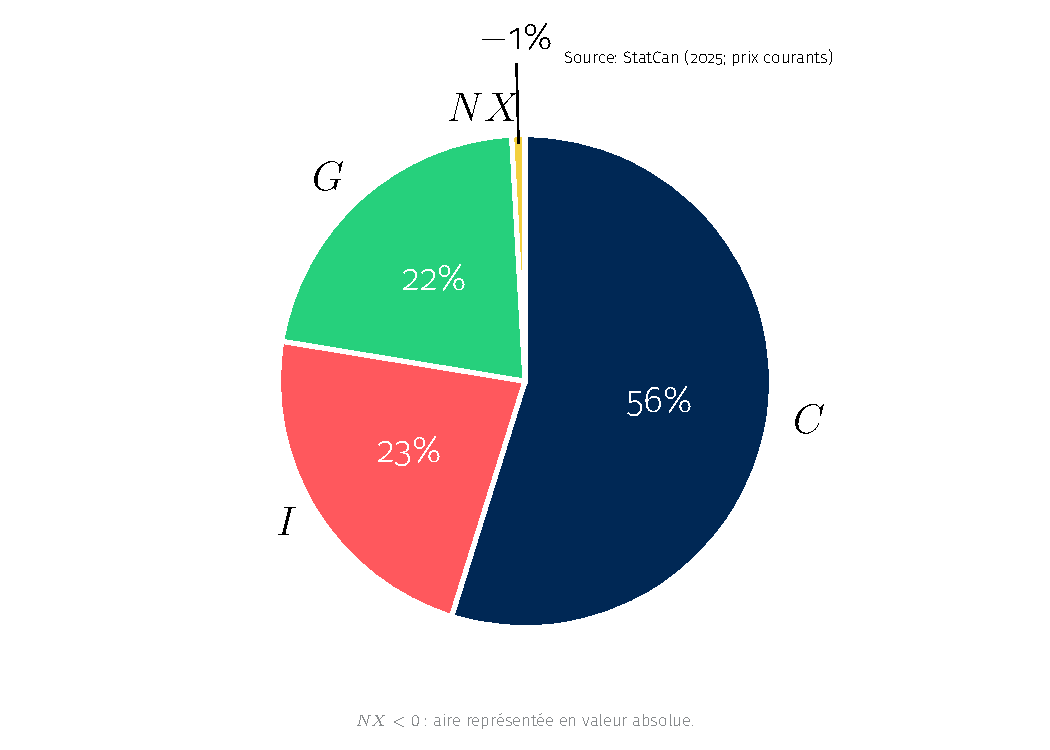
\includegraphics[height=0.8\textheight]{gdp_decomposition_canada.pdf}
   \end{figure}
\end{frame}

% ============================================================================
% 10 | \begin{frame}[t]{Consommation ($C$)}
% Source: S1/s1.tex | \begin{frame}[t]{Consommation ($C$)}
% ============================================================================
\begin{frame}[t]{Consommation ($C$)}
   \textbf{Dépenses des ménages} en biens et services finaux :
   \vspace{0.2cm}
   \begin{itemize}
      \setlength\itemsep{0.2cm}
      \item \textbf{Biens durables} --- voitures, meubles, électroménagers (longue vie utile)
      \item \textbf{Biens non durables} --- alimentation, vêtements, essence (courte vie utile)
      \item \textbf{Services} --- loyer, soins de santé, coiffure, éducation
   \end{itemize}
   \vspace{0.3cm}
   \begin{keyinsight}
      Les services représentent plus de 60\,\% de la consommation au Canada. Ce virage vers les services caractérise les économies avancées.
   \end{keyinsight}
\end{frame}

% ============================================================================
% 11 | \begin{frame}[t]{Investissement ($I$)}
% Source: S1/s1.tex | \begin{frame}[t]{Investissement ($I$)}
% ============================================================================
\begin{frame}[t]{Investissement ($I$)}
   \textbf{Dépenses en biens destinés à produire dans le futur :}
   \vspace{0.2cm}
   \begin{itemize}
      \setlength\itemsep{0.2cm}
      \item \textbf{Capital fixe des entreprises} --- machines, équipements, usines, logiciels
      \item \textbf{Résidentiel} --- construction de nouveaux logements
      \item \textbf{Stocks} --- biens invendus entreposés
   \end{itemize}
   \vspace{0.3cm}
   \begin{warning}[Confusion fréquente]
      En économie, \guillemotleft~investissement~\guillemotright\ $=$ \textbf{formation de capital physique}, pas l'achat de titres financiers. Acheter un camion de livraison $=$ investissement; acheter des actions de Tesla, non.
   \end{warning}
\end{frame}

% ============================================================================
% 12 | \begin{frame}[t]{Dépenses gouvernementales ($G$)}
% Source: S1/s1.tex | \begin{frame}[t]{Dépenses gouvernementales ($G$)}
% ============================================================================
\begin{frame}[t]{Dépenses gouvernementales ($G$)}
   \small
   Le gouvernement est un producteur \textbf{majeur} de biens et services :
   \vspace{0.05cm}
   \begin{itemize}
      \footnotesize
      \setlength\itemsep{0.05cm}
      \item Défense, éducation, santé, police, justice, pompiers, etc.
      \item Infrastructures (routes, ponts, transport en commun) selon NIPA ($G$) vs.\ SNA ($I$)
   \end{itemize}
   \vspace{0.15cm}
   \begin{defbox}[Évalué au coût]
      Souvent sans prix de marché, donc $G$ est mesuré par le \textbf{coût des intrants}.
   \end{defbox}
   \vspace{0.1cm}
   \begin{warning}[Transferts $\neq$ dépenses gouvernementales]
      Les transferts (assurance-emploi, pensions, aide sociale) ne font \textbf{pas} partie de $G$ : ils redistribuent le revenu existant, sans nouvelle production.
   \end{warning}
\end{frame}

% ============================================================================
% 13 | \begin{frame}[t]{Exportations et importations ($NX$)}
% Source: S1/s1.tex | \begin{frame}[t]{Exportations et importations ($NX$)}
% ============================================================================
\begin{frame}[t]{Exportations et importations ($NX$)}
   $C$, $I$ et $G$ incluent les dépenses en biens \textbf{étrangers} (importations).\\[4pt]
   Puisque le PIB mesure la production \textit{intérieure}, il faut une correction :
   \vspace{0.1cm}
   \begin{equation*}
      Y = \underbrace{C + I + G}_{\text{dépenses totales}} + \underbrace{X - M}_{\text{export.\ nettes}}
   \end{equation*}
   \vspace{-0.3cm}
   \begin{itemize}
      \setlength\itemsep{0.1cm}
      \item $X$ (exportations) : production intérieure vendue à l'étranger
      \item $M$ (importations) : production étrangère déjà comptée dans $C$, $I$, $G$
   \end{itemize}
   \vspace{0.15cm}
   \begin{defbox}[Ouverture commerciale]
      $(X + M) / Y$ mesure l'importance du commerce pour une économie.
   \end{defbox}
\end{frame}

% ============================================================================
% 14 | \begin{frame}{PIB par les dépenses : comparaison internationale}
% Source: S1/s1.tex | \begin{frame}{PIB par les dépenses : comparaison internationale}
% ============================================================================
\begin{frame}{PIB par les dépenses : comparaison internationale}
   \vspace{-0.15cm}
   \begin{figure}
      \centering
      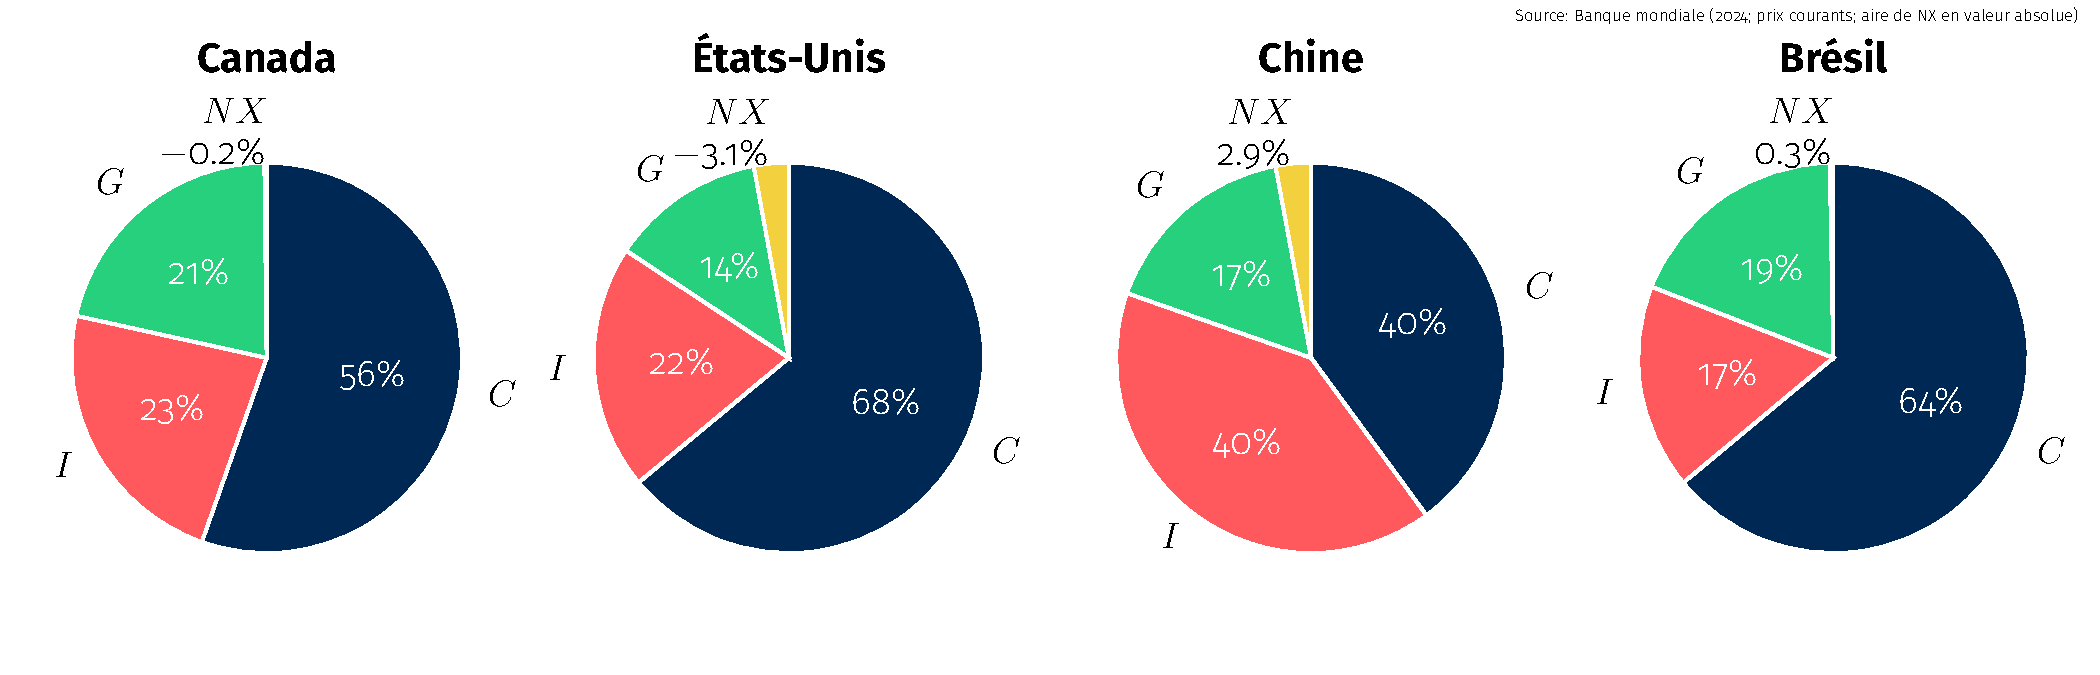
\includegraphics[width=\textwidth, height=0.62\textheight, keepaspectratio]{gdp_decomposition_4countries.pdf}
   \end{figure}
   \vspace{-0.25cm}
   \begin{keyinsight}[Différents modèles de croissance]
      Chine : investissement ($I$ = 40\,\%). É.-U.\ : consommation ($C$ = 68\,\%).
   \end{keyinsight}
\end{frame}

% ============================================================================
% 15 | \begin{frame}{Croissance du PIB nominal vs.\ réel au Canada}
% Source: S1/s1.tex | \begin{frame}{Croissance du PIB nominal vs.\ réel au Canada}
% ============================================================================
\begin{frame}{Croissance du PIB nominal vs.\ réel au Canada}
   \begin{figure}
      \centering
      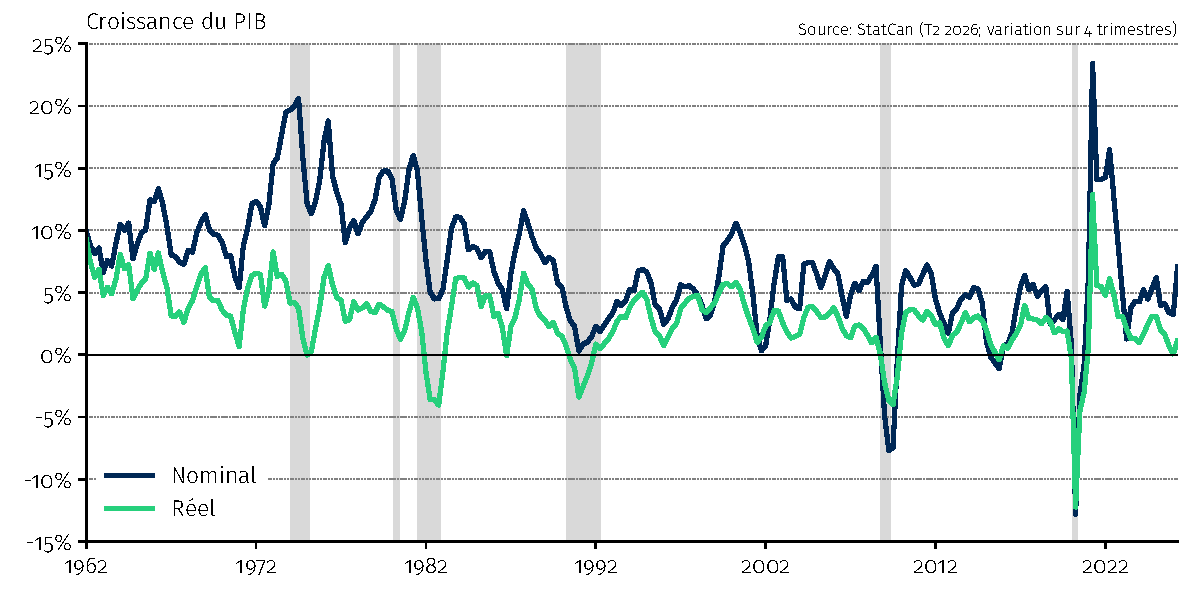
\includegraphics[width=\textwidth]{gdp_nominal_real_canada.pdf}
   \end{figure}
\end{frame}

% ============================================================================
% 16 | \begin{frame}[t]{PIB et prix}
% Source: S1/s1.tex | \begin{frame}[t]{PIB et prix}
% Adaptation: Math-source product convention only.
% ============================================================================
\begin{frame}[t]{PIB et prix}
   \begin{defbox}
      \vspace{-0.5cm}
      \begin{itemize}
         \setlength\itemsep{0.15cm}
         \item \textbf{PIB nominal} = production évaluée aux prix \textit{courants}
         \item \textbf{PIB réel} = production évaluée à prix \textit{constants} (année de référence)
         \item \textbf{Déflateur du PIB} = $\frac{\text{PIB nominal}}{\text{PIB réel}} \cdot 100$
      \end{itemize}
   \end{defbox}
   \vspace{0.05cm}
   \begin{keyinsight}
      Le PIB nominal est contaminé par les variations de prix. Le PIB réel isole les variations de quantité, mesurant la vraie croissance de la \textit{production}.
   \end{keyinsight}
\end{frame}

% ============================================================================
% 17 | \begin{frame}{Qu'est-ce que l'inflation\,?}
% Source: S1/s1.tex | \begin{frame}{Qu'est-ce que l'inflation\,?}
% Adaptation: Make percentage units explicit.
% ============================================================================
\begin{frame}{Qu'est-ce que l'inflation\,?}
   \begin{defbox}[Inflation]
      Le taux de variation en \% du \textbf{niveau général des prix} entre deux périodes.
   \end{defbox}

   \begin{equation*}
      \pi_t = \frac{P_t - P_{t-1}}{P_{t-1}} \cdot 100 = \%\Delta P \quad \text{où $P_t =$ niveau des prix au temps $t$}
   \end{equation*}

   \vspace{0.3cm}

   \textbf{Question clé :} comment mesurer $P_t$\,?
   \vspace{0.2cm}
   \begin{itemize}
      \setlength\itemsep{0.15cm}
      \item \textbf{Déflateur du PIB :} prix de tous les biens produits domestiquement (large)
      \item \textbf{Indice des prix à la consommation (IPC) :} prix d'un panier de biens de consommation (le plus courant)
   \end{itemize}
\end{frame}

% ============================================================================
% 18 | \begin{frame}{Inflation globale vs.\ de base}
% Source: S1/s1.tex | \begin{frame}{Inflation globale vs.\ de base}
% ============================================================================
\begin{frame}{Inflation globale vs.\ de base}
   \begin{figure}
      \centering
      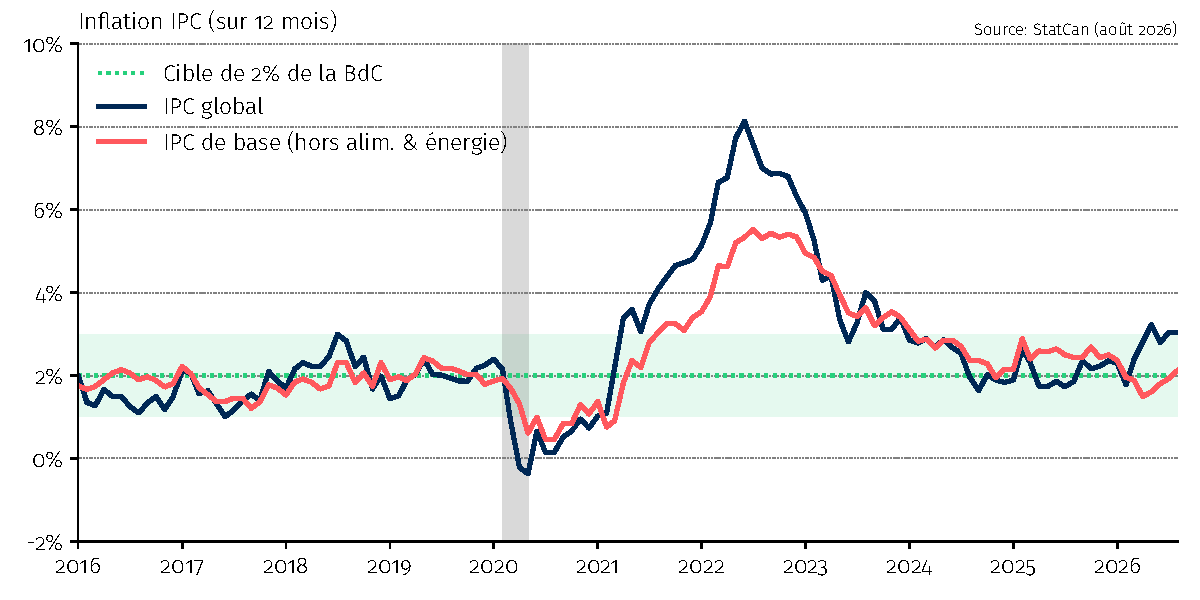
\includegraphics[width=0.95\textwidth, height=0.75\textheight, keepaspectratio]{inflation_headline_core_canada.pdf}
   \end{figure}
\end{frame}

% ============================================================================
% 19 | \begin{frame}[t]{PIB réel vs.\ PIB réel par habitant}
% Source: S1/s1.tex | \begin{frame}[t]{PIB réel vs.\ PIB réel par habitant}
% ============================================================================
\begin{frame}[t]{PIB réel vs.\ PIB réel par habitant}
   \small
   \begin{itemize}
      \setlength\itemsep{0.15cm}
      \item Le \textbf{PIB réel} mesure la taille totale de l'économie
      \item Le \textbf{PIB réel par habitant} mesure le niveau de vie moyen
   \end{itemize}
   \vspace{0.1cm}
   \begin{bizimplication}[Stratégie de marché]
      \small Vous vendez des sacs à main de luxe. Viser un pays au PIB élevé ou au PIB par habitant élevé\,? Et si vous vendez des biens abordables à faibles marges\,?
   \end{bizimplication}
   \vspace{0.1cm}
   \begin{bizimplication}[Rémunération]
      \small Vos employés demandent une hausse car \guillemotleft~l'économie croît~\guillemotright. Le PIB a progressé de 15\,\% en 10 ans. Bon argument pour de meilleurs salaires\,?
   \end{bizimplication}
\end{frame}

% ============================================================================
% 20 | \begin{frame}[t]{Trois catégories}
% Source: S3/s3.tex | \begin{frame}[t]{Trois catégories}
% ============================================================================
\begin{frame}[t]{Trois catégories}
   \small
   La population en âge de travailler se divise en trois groupes :
   \vspace{0.2cm}
   \begin{center}
   \begin{tikzpicture}[
      node distance=1.5cm,
      box/.style={draw=HECnavy, rounded corners=6pt, thick, minimum width=3cm,
                  minimum height=1cm, align=center, font=\small\bfseries},
      arr/.style={-{Stealth[length=5pt]}, thick, HECgray}
   ]
      \node[box, fill=HECgreen!10] (E) {Employés\\($E$)};
      \node[box, fill=HECcoral!10, right=2.5cm of E] (U) {Chômeurs\\($U$)};
      \node[box, fill=HEClightgray, below=1.5cm of $(E)!0.5!(U)$] (I) {Inactifs\\($I$)};

      \draw[arr, bend left=15] (E) to node[above, font=\scriptsize] {licenciement/départ} (U);
      \draw[arr, bend left=15] (U) to node[above, font=\scriptsize] {embauche} (E);
      \draw[arr, bend left=15] (U) to node[right, font=\scriptsize] {découragement} (I);
      \draw[arr, bend left=15] (I) to node[left, font=\scriptsize] {retour} (U);
      \draw[arr, bend right=15] (E) to node[left, font=\scriptsize] {retraite} (I);
   \end{tikzpicture}
   \end{center}
   \begin{defbox}
      \RaggedRight
      \textbf{Chômeur :} sans emploi, disponible et en \textbf{recherche active}.
   \end{defbox}
\end{frame}

% ============================================================================
% 21 | \begin{frame}[t]{Trois ratios essentiels}
% Source: S3/s3.tex | \begin{frame}[t]{Trois ratios essentiels}
% ============================================================================
\begin{frame}[t]{Trois ratios essentiels}
   \begin{defbox}[Indicateurs du marché du travail]
      \RaggedRight
      \vspace{-0.5cm}
      \begin{align*}
         \text{Taux de participation} &= \frac{E + U}{\text{Pop.\ en âge de travailler}} \times 100 \\[5pt]
         \text{Taux d'emploi} &= \frac{E}{\text{Pop.\ en âge de travailler}} \times 100 \\[5pt]
         \text{Taux de chômage} &= \frac{U}{E + U} \times 100
      \end{align*}
   \end{defbox}
\end{frame}

% ============================================================================
% 22 | \begin{frame}{Le marché du travail canadien}
% Source: S3/s3.tex | \begin{frame}{Le marché du travail canadien}
% ============================================================================
\begin{frame}{Le marché du travail canadien}
   \begin{figure}
      \centering
      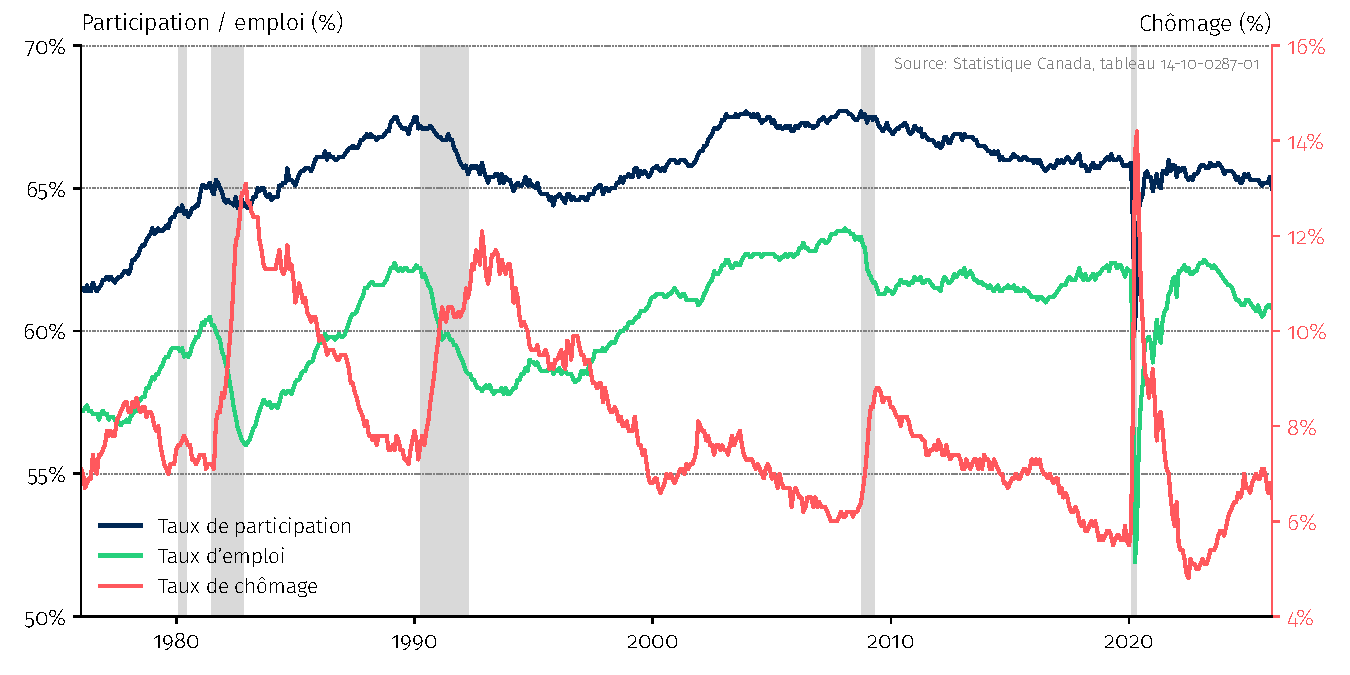
\includegraphics[width=0.95\textwidth]{labor_market_indicators_ca.pdf}
   \end{figure}
\end{frame}

% ============================================================================
% 23 | \begin{frame}[t]{Pourquoi le taux de chômage ne suffit-il pas\,?}
% Source: S3/s3.tex | \begin{frame}[t]{Pourquoi le taux de chômage ne suffit-il pas\,?}
% ============================================================================
\begin{frame}[t]{Pourquoi le taux de chômage ne suffit-il pas\,?}
   \footnotesize
   \vspace{-0.2cm}
   \begin{warning}[Limites du taux de chômage]
      \RaggedRight
      \vspace{-0.4cm}
      \begin{itemize}
         \setlength\itemsep{0.07cm}
         \item \textbf{Travailleurs découragés :} une baisse du chômage peut refléter des \textit{retraits} du marché, non pas des embauches
         \item \textbf{Sous-emploi :} travail à temps partiel faute de trouver un emploi à temps plein
         \item \textbf{Qualité des emplois :} un taux très faible peut signifier que les travailleurs n'ont pas les ressources pour chercher assez longtemps afin de trouver un bon \textit{match}
         \item \textbf{Démographie :} les départs à la retraite réduisent la participation; le taux de chômage ne résume pas cet effet
      \end{itemize}
   \end{warning}
   \vspace{0.05cm}
   \begin{bizimplication}
      \RaggedRight
      Pour évaluer la santé réelle du marché du travail, regardez le taux de participation, le taux d'emploi \textbf{et} les mesures de sous-emploi (U-6 aux États-Unis).
   \end{bizimplication}
\end{frame}

% ============================================================================
% 24 | \begin{frame}[t]{Ce que le PIB ne mesure \textit{pas}}
% Source: S1/s1.tex | \begin{frame}[t]{Ce que le PIB ne mesure \textit{pas}}
% Adaptation: Correct Italy revision magnitude and clarify partially measured activity.
% ============================================================================
\begin{frame}[t]{Ce que le PIB ne mesure \textit{pas}}
   Le PIB omet une partie de l’activité économique ou la mesure imparfaitement :
   \vspace{0.2cm}
   \begin{itemize}
      \setlength\itemsep{0.15cm}
      \item \textbf{Production domestique} --- cuisine, garde d'enfants, réparations à domicile
      \item \textbf{Bénévolat} --- services communautaires, organismes de bienfaisance
      \item \textbf{Économie souterraine} --- revenus non déclarés, travail informel : estimés en partie
   \end{itemize}
   \vspace{0.2cm}
   \begin{keyinsight}[Sexe, drogues et PIB]
      En 2014, l'Italie a intégré certaines activités illégales (drogues, prostitution, contrebande) dans ses comptes nationaux : environ 1\,\% de PIB mesuré en plus pour 2011.
      \hfill{\scriptsize\textit{\color{black!50}\href{https://www.istat.it/wp-content/uploads/2024/01/Alleva_National-Accounts_-27112017.pdf}{ISTAT, 2017, p.\ 9}}}
   \end{keyinsight}
\end{frame}

% ============================================================================
% 25 | \begin{frame}[t]{Où trouver l'information économique\,?}
% Source: Programme-specific resource guide; destinations checked 2026-10-26.
% Replaces the Jones--Tonetti scenario slide, after the indicators section.
% ============================================================================
\begin{frame}[t]{Où trouver l'information économique\,?}
   \small
   \renewcommand{\arraystretch}{1.2}
   \begin{tabularx}{\textwidth}{@{}>{\bfseries\raggedright\arraybackslash}p{0.26\textwidth}J@{}}
      \textcolor{HECnavy}{Canada et Québec} &
      \href{https://www.statcan.gc.ca/fr/debut}{Statistique Canada},
      \href{https://statistique.quebec.ca/fr}{Institut de la statistique du Québec},
      \href{https://www.banqueducanada.ca/}{Banque du Canada} \\
      \addlinespace[14pt]
      \textcolor{HECnavy}{International} &
      \href{https://fred.stlouisfed.org/}{FRED},
      \href{https://www.oecd.org/fr.html}{OCDE},
      \href{https://www.imf.org/fr/home}{FMI},
      \href{https://donnees.banquemondiale.org/}{Banque mondiale},
      \href{https://ourworldindata.org/}{Our World in Data} \\
      \addlinespace[14pt]
      \textcolor{HECnavy}{Presse} &
      \href{https://www.ft.com/}{\textit{Financial Times}},
      \href{https://www.economist.com/}{\textit{The Economist}},
      \href{https://www.wsj.com/}{\textit{The Wall Street Journal}} \\
      \addlinespace[14pt]
      \textcolor{HECnavy}{Blogues et balados} &
      \href{https://www.grumpy-economist.com/}{\textit{The Grumpy Economist}} (John H.\ Cochrane),
      \href{https://marginalrevolution.com/}{\mbox{\textit{Marginal Revolution}}},
      \href{https://freakonomics.com/podcasts/}{\mbox{\textit{Freakonomics Radio}}}
   \end{tabularx}
   \vspace{0.10cm}
   \begin{keyinsight}[Lire avec recul]
      \small\RaggedRight
      Vérifiez la \textbf{date}, les \textbf{unités} et les \textbf{révisions}. Distinguez \textbf{données}, \textbf{prévisions} et \textbf{opinions}; croisez les sources.
   \end{keyinsight}
\end{frame}

% ============================================================================
% 26 | \sectionframe{Production et croissance\\Travail, capital et IA}
% Source: Shared ECON50803 title/section style
% ============================================================================
\sectionframe{Production et croissance\\Travail, capital et IA}

% ============================================================================
% 27 | \begin{frame}{La croissance est un phénomène récent}
% Source: S2/s2.tex | \begin{frame}{La croissance est un phénomène récent}
% ============================================================================
\begin{frame}{La croissance est un phénomène récent}
   \begin{figure}
      \centering
      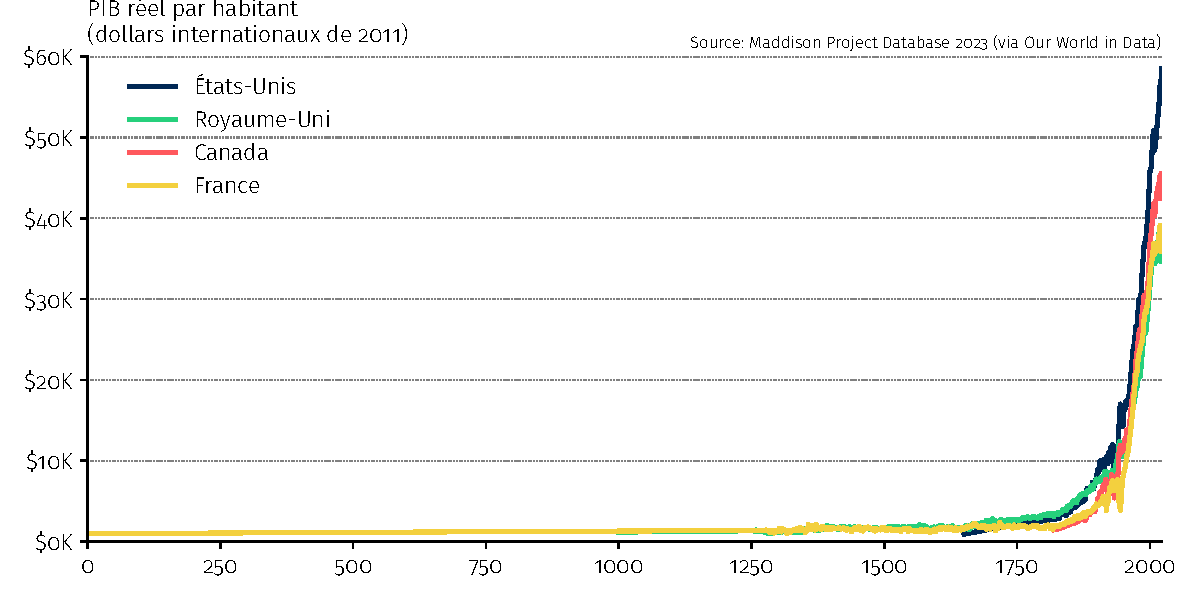
\includegraphics[width=0.95\textwidth]{hockey_stick_world.pdf}
   \end{figure}
\end{frame}

% ============================================================================
% 28 | \begin{frame}[t]{Quels sont les ingrédients\,?}
% Source: S2/s2.tex | \begin{frame}[t]{Quels sont les ingrédients\,?}
% ============================================================================
\begin{frame}[t]{Quels sont les ingrédients\,?}
   \vfill
   \begin{columns}[c]
      \begin{column}{0.30\textwidth}
         \centering
         {\large\textbf{\textcolor{HECnavy}{Capital ($K$)}}}\\[8pt]
         \footnotesize
         Machines, équipements,\\bâtiments, infrastructures
      \end{column}
      \begin{column}{0.40\textwidth}
         \centering
         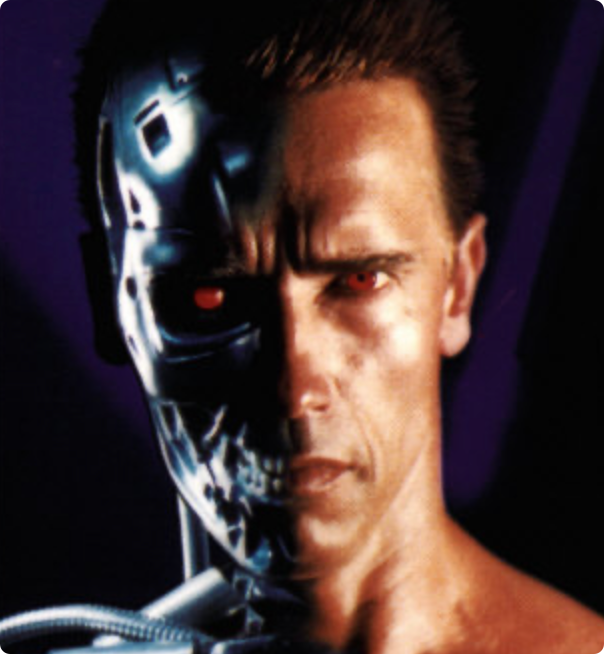
\includegraphics[width=\textwidth, keepaspectratio]{terminator.png}
      \end{column}
      \begin{column}{0.30\textwidth}
         \centering
         {\large\textbf{\textcolor{HECnavy}{Travail ($L$)}}}\\[8pt]
         \footnotesize
         Heures travaillées,\\nombre d'employés
      \end{column}
   \end{columns}
   \vfill
\end{frame}

% ============================================================================
% 29 | \begin{frame}{Le vieillissement de la population}
% Source: S3/s3.tex | \begin{frame}{Le vieillissement de la population}
% ============================================================================
\begin{frame}{Le vieillissement de la population}
   \begin{figure}
      \centering
      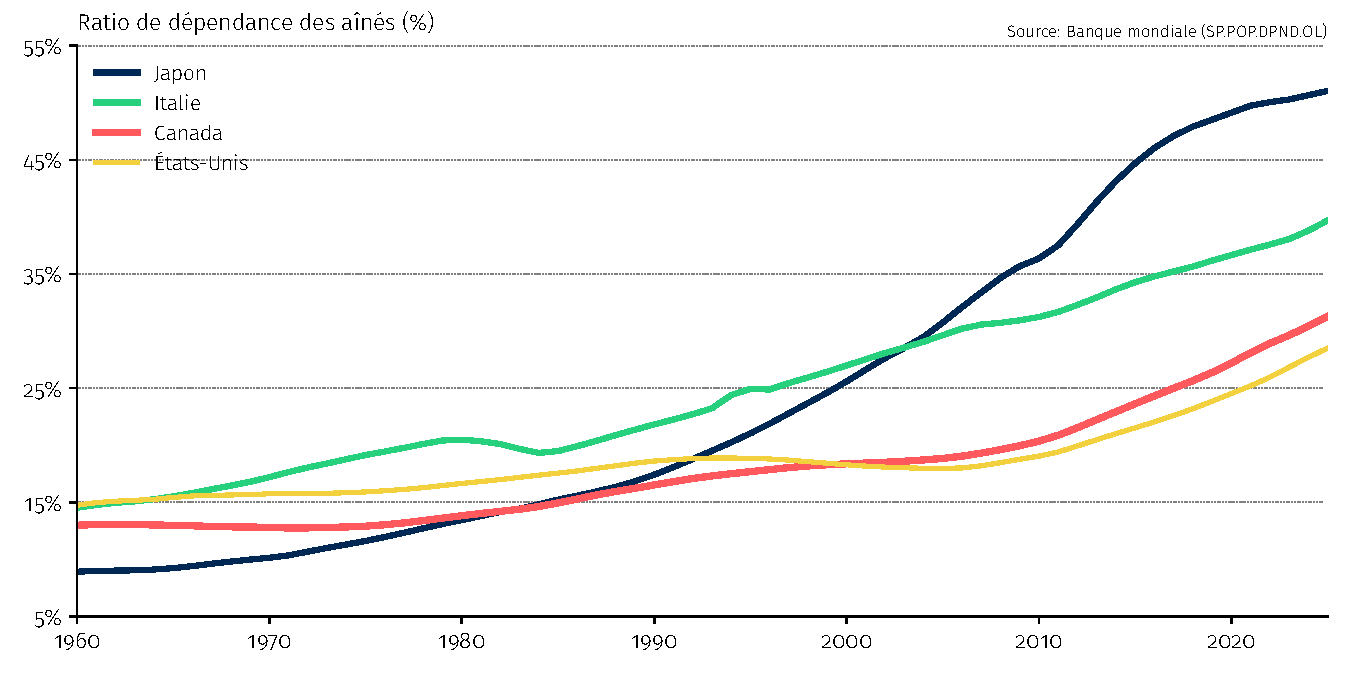
\includegraphics[width=0.95\textwidth]{aging_population.pdf}
   \end{figure}
\end{frame}

% ============================================================================
% 30 | \begin{frame}[t]{L'équilibre de plein emploi}
% Source: S3/s3.tex | \begin{frame}[t]{L'équilibre de plein emploi}
% ============================================================================
\begin{frame}[t]{L'équilibre de plein emploi}
   \begin{columns}[T]
      \begin{column}{0.48\textwidth}
         L'intersection donne :
         \vspace{0.15cm}
         \begin{itemize}
            \setlength\itemsep{0.15cm}
            \item $L^* =$ emploi d'équilibre
            \item $w^* =$ salaire \textit{réel} d'équilibre
         \end{itemize}
         \vspace{0.2cm}
         \begin{keyinsight}
            \RaggedRight
            À l'équilibre, le salaire s'ajuste de sorte que ceux qui veulent travailler trouvent un emploi.
         \end{keyinsight}
      \end{column}
      \begin{column}{0.48\textwidth}
         \centering
         \begin{tikzpicture}[scale=0.9]
            \draw[refline] (2.32,0) node[below, pointlabel] {$L^*$} -- (2.32,2.06);
            \draw[refline] (0,2.06) node[left, pointlabel] {$w^*$} -- (2.32,2.06);
            % Supply: y = 0.857x + 0.074. Y-int (0,0.07). At x=4.7: y=4.10
            \draw[supply] (0,0.07) -- (4.7,4.10) node[right, curvelabel] {$L^S$};
            % Demand: y = -0.927x + 4.213. Y-int (0,4.21). X-int (4.54,0)
            \draw[demand] (0,4.21) -- (4.54,0) node[above right, curvelabel] {$L^D$};
            % Intersection at (2.32, 2.06)
            \filldraw[eqpoint] (2.32,2.06) circle (3pt);
            \draw[econaxis] (0,0) -- (5,0) node[right] {$L$};
            \draw[econaxis] (0,0) -- (0,4.5) node[above] {$w$};
         \end{tikzpicture}
      \end{column}
   \end{columns}
\end{frame}

% ============================================================================
% 31 | \begin{frame}[t]{Capital, investissement et financement}
% Source: S3/s3.tex | \begin{frame}[t]{Capital, investissement et financement}
% ============================================================================
\begin{frame}[t]{Capital, investissement et financement}
\begin{defbox}[Stock vs.\ flux]
   \RaggedRight
      \textbf{Capital ($K$)} : machines, bâtiments, logiciels déjà en place\\[5pt]
      \textbf{Investissement ($I$)} : production de nouveaux actifs
   \end{defbox}
   \vspace{0.3cm}
   \textbf{Exemple :} une entreprise construit une usine et émet des obligations.
   \begin{itemize}
      \setlength\itemsep{0.15cm}
      \item La construction de l'usine est un \textbf{investissement}.
      \item L'émission d'obligations est son \textbf{financement}.
   \end{itemize}
   \vspace{0.2cm}
   Acheter une action existante ne crée pas directement du nouveau capital.
\end{frame}

% ============================================================================
% 32 | \begin{frame}[t]{Rendements décroissants : capital}
% Source: S2/s2.tex | \begin{frame}[t]{Rendements décroissants : capital}
% ============================================================================
\begin{frame}[t]{Rendements décroissants : capital}
   \begin{columns}[c]
      \begin{column}{0.58\textwidth}
         \centering
         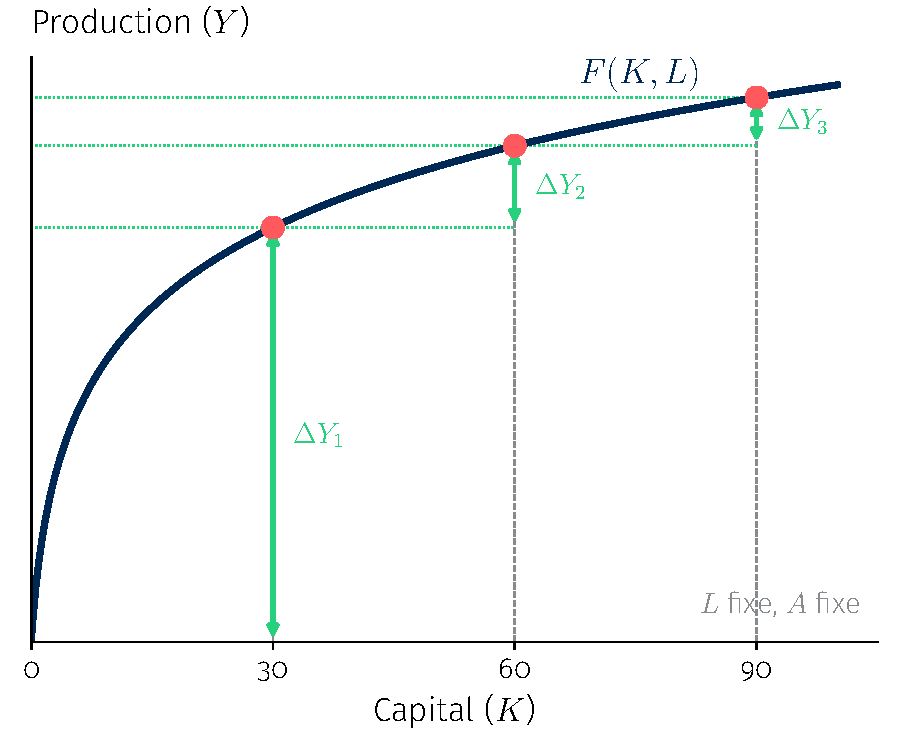
\includegraphics[width=\textwidth]{production_function_capital.pdf}
      \end{column}
      \begin{column}{0.40\textwidth}
         \small
         À travail fixe, chaque machine supplémentaire \textbf{ajoute de moins en moins} à la production.
         \vspace{0.3cm}

         \textbf{Analogie :} donner 10 ordinateurs à un seul employé --- le 10\textsuperscript{e} n'aide plus du tout\,!
         \vspace{0.3cm}

         \begin{warning}
            \small Plus de $K$ $\to$ plus de $Y$, mais à un rythme \textbf{décroissant}
         \end{warning}
      \end{column}
   \end{columns}
\end{frame}

% ============================================================================
% 33 | \begin{frame}[t]{Qu'est-ce que la PTF ($A$)\,?}
% Source: S2/s2.tex | \begin{frame}[t]{Qu'est-ce que la PTF ($A$)\,?}
% ============================================================================
\begin{frame}[t]{Qu'est-ce que la PTF ($A$)\,?}
   \small
   Deux boulangeries avec les \textbf{mêmes ingrédients} (farine, beurre, œufs, employés).
   \vspace{0.25cm}
   \begin{columns}[T]
      \begin{column}{0.47\textwidth}
         \centering
         \textcolor{HECgray}{\large\textbf{Boulangerie \#1}}\\[3pt]
         \textcolor{HECgray}{PTF faible}\\[4pt]
         \footnotesize
         Recettes de base\\
         Fours mal calibrés\\
         Organisation chaotique\\[4pt]
         $\to$ 100 pains / jour
      \end{column}
      \begin{column}{0.06\textwidth}
         \centering
         \vspace{0.8cm}
         {\Large\textcolor{HECgray}{vs}}
      \end{column}
      \begin{column}{0.47\textwidth}
         \centering
         \textcolor{HECgreen}{\large\textbf{Boulangerie \#2}}\\[3pt]
         \textcolor{HECgreen}{PTF élevée}\\[4pt]
         \footnotesize
         Techniques de levain maîtrisées\\
         Fours optimisés\\
         Processus rodé\\[4pt]
         $\to$ 200 pains / jour
      \end{column}
   \end{columns}
   \vspace{0.25cm}
   \begin{keyinsight}
      La PTF ($A$) capte \textbf{tout ce qui n'est pas $K$ ou $L$} : technologie, savoir-faire, gestion, organisation\ldots\ C'est la capacité à faire \textbf{plus avec les mêmes ressources}.
   \end{keyinsight}
\end{frame}

% ============================================================================
% 34 | \begin{frame}{Décomposition de la croissance canadienne}
% Source: S2/s2.tex | \begin{frame}{Décomposition de la croissance canadienne}
% ============================================================================
\begin{frame}{Décomposition de la croissance canadienne}
   \begin{figure}
      \centering
      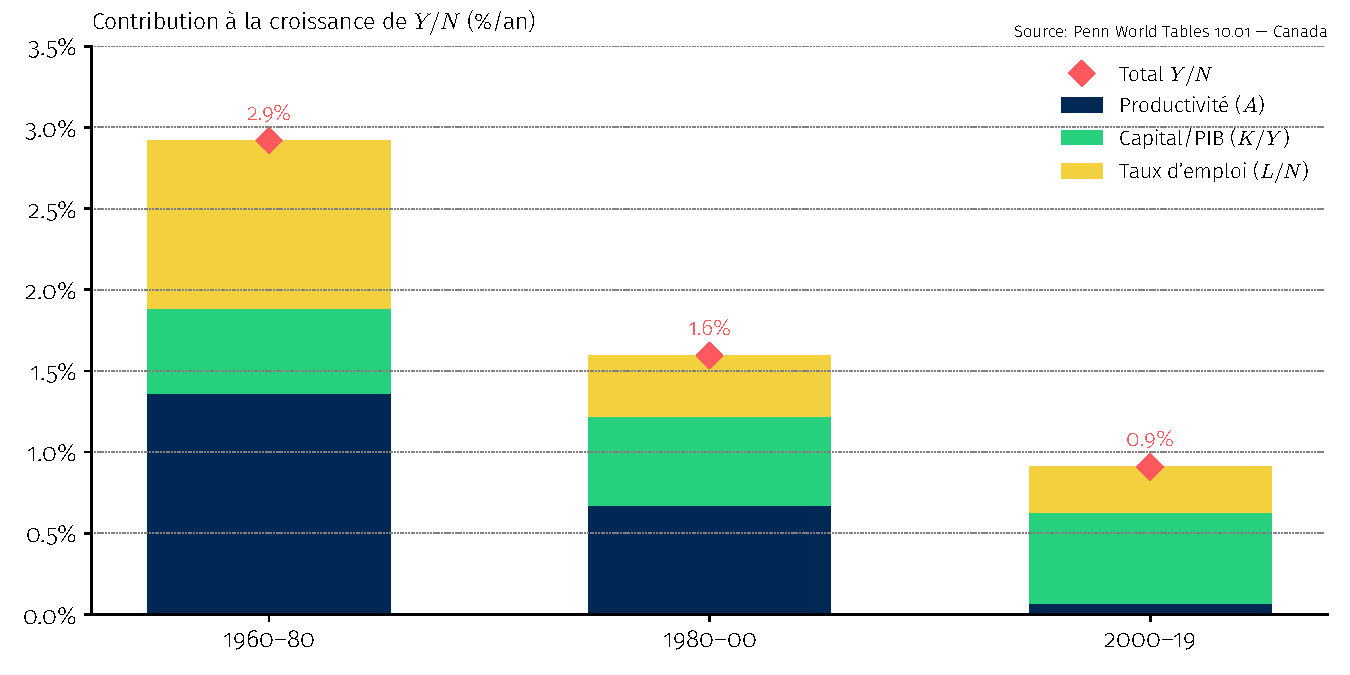
\includegraphics[width=0.95\textwidth, keepaspectratio]{canada_gdp_decomposition.pdf}
   \end{figure}
\end{frame}

% ============================================================================
% 35 | \begin{frame}[t]{Sommaire : théories de la productivité}
% Source: S2/s2.tex | \begin{frame}[t]{Sommaire : théories de la productivité}
% ============================================================================
\begin{frame}[t]{Sommaire : théories de la productivité}
   \small
   \vspace{0.1cm}
   La croissance à l'échelle mondiale peut être caractérisée par\ldots
   \begin{columns}[T,onlytextwidth]
      \begin{column}{0.30\textwidth}
         \begin{tcolorbox}[colback=HECgreen!8, colframe=HECgreen, boxrule=0.5pt, arc=8pt,
            top=4pt, bottom=4pt, left=6pt, right=6pt]
            \centering\footnotesize\textbf{Économies matures}\\[3pt]
            En ralentissement\ldots
         \end{tcolorbox}
      \end{column}
      \begin{column}{0.30\textwidth}
         \begin{tcolorbox}[colback=HECnavy!8, colframe=HECnavy, boxrule=0.5pt, arc=8pt,
            top=4pt, bottom=4pt, left=6pt, right=6pt]
            \centering\footnotesize\textbf{Économies émergentes}\\[3pt]
            En rattrapage\ldots
         \end{tcolorbox}
      \end{column}
      \begin{column}{0.30\textwidth}
         \begin{tcolorbox}[colback=HECcoral!8, colframe=HECcoral, boxrule=0.5pt, arc=8pt,
            top=4pt, bottom=4pt, left=6pt, right=6pt]
            \centering\footnotesize\textbf{Économies stagnantes}\\[3pt]
            Peinent à décoller\ldots
         \end{tcolorbox}
      \end{column}
   \end{columns}
   \vspace{0.25cm}
   Le succès repose sur des \textbf{conditions appropriées} :
   \vspace{0.1cm}
   \begin{itemize}
      \setlength\itemsep{0.1cm}
      \item La prospérité coïncide rarement avec un contexte institutionnel faible
      \item Des institutions inclusives encouragent l'innovation et la productivité
   \end{itemize}
   \vspace{0.1cm}
   \begin{bizimplication}[Expansion internationale]
      \footnotesize La qualité institutionnelle compte autant que la taille du marché.
   \end{bizimplication}
\end{frame}

% ============================================================================
% 36 | \begin{frame}[t]{Qui épargne\,?}
% Source: S3/s3.tex | \begin{frame}[t]{Qui épargne\,?}
% ============================================================================
\begin{frame}[t]{Qui épargne\,?}
   \begin{defbox}[Épargne nationale]
      \RaggedRight
      \vspace{-0.25cm}
      \begin{equation*} S = S_P + S_G \end{equation*}
      La part du revenu qui n'est pas consommée.
   \end{defbox}
   \vspace{0.25cm}
   \begin{itemize}
      \setlength\itemsep{0.3cm}
      \item \textbf{Épargne privée ($S_P$) :} ménages et entreprises.
      \item \textbf{Épargne publique ($S_G$) :} dans le modèle, $S_G = T - G$.
   \end{itemize}
   \vspace{0.3cm}
   {\small $T$ : impôts nets des transferts; $G$ : consommation publique.\\[4pt]
   L'investissement public fait partie de $I$, pas de $G$.}
\end{frame}

% ============================================================================
% 37 | \begin{frame}[t]{Équilibre en économie fermée}
% Source: S3/s3.tex | \begin{frame}[t]{Équilibre en économie fermée}
% ============================================================================
\begin{frame}[t]{Équilibre en économie fermée}
\begin{columns}[c]
      \begin{column}{0.53\textwidth}
         \centering
         \begin{tikzpicture}[scale=.78]
\draw[refline] (3,0) node[below, pointlabel] {$I_0$} -- (3,2.25);
       \draw[refline] (0,2.25) node[left, pointlabel] {$r_0$} -- (3,2.25);
\draw[very thick, HECnavy] (0,0) -- (6.4,4.8) node[right, curvelabel] {$S$};
       \draw[very thick, HECcoral] (0,4.5) -- (6,0) node[above right, curvelabel] {$I$};
\filldraw[eqpoint] (3,2.25) circle (3pt);
       \draw[econaxis] (0,0) -- (7.4,0) node[right] {$S, I$};
       \draw[econaxis] (0,0) -- (0,6) node[above] {$r$};
    \end{tikzpicture}
      \end{column}
      \begin{column}{0.43\textwidth}
         \small

   \textbf{Sans financement extérieur :}
   \begin{itemize}
      \setlength\itemsep{0.2cm}
      \item Les projets n'utilisent que l'épargne nationale.
      \item Le taux d'intérêt \textbf{réel} s'ajuste.
      \item À l'équilibre, $S = I$.
   \end{itemize}
   \vspace{0.2cm}
   \begin{keyinsight}
      \RaggedRight
      Si les projets désirés dépassent l'épargne offerte, $r$ augmente.
   \end{keyinsight}
      \end{column}
   \end{columns}
\end{frame}

% ============================================================================
% 38 | \begin{frame}[t]{Faut-il se limiter à l'épargne canadienne\,?}
% Source: S3/s3.tex | \begin{frame}[t]{Faut-il se limiter à l'épargne canadienne\,?}
% ============================================================================
\begin{frame}[t]{Faut-il se limiter à l'épargne canadienne\,?}
\vspace{0.2cm}
   Une entreprise canadienne peut financer son usine auprès d'un \textbf{fonds de pension allemand} ou d'un \textbf{investisseur japonais}.
   \vspace{0.4cm}
   \begin{itemize}
      \setlength\itemsep{0.25cm}
      \item Le Canada peut investir \textbf{plus} que son épargne nationale.
      \item Les Canadiens peuvent aussi financer des projets à l'étranger.
      \item Le coût du financement dépend des conditions \textbf{mondiales}.
   \end{itemize}
   \vspace{0.3cm}
   \begin{keyinsight}
      \RaggedRight
      Ouvrir l'économie permet de dissocier l'épargne nationale et l'investissement domestique.
   \end{keyinsight}
\end{frame}

% ============================================================================
% 39 | \begin{frame}[t]{Que prévoient les entreprises pour l'emploi\,?}
% Source: S3/s3.tex | \begin{frame}[t]{Que prévoient les entreprises pour l'emploi\,?}
% ============================================================================
\begin{frame}[t]{Que prévoient les entreprises pour l'emploi\,?}
   \framesubtitle{Baslandze et al. (2026) : 734 dirigeants financiers américains interrogés fin 2025.}
   {\centering
   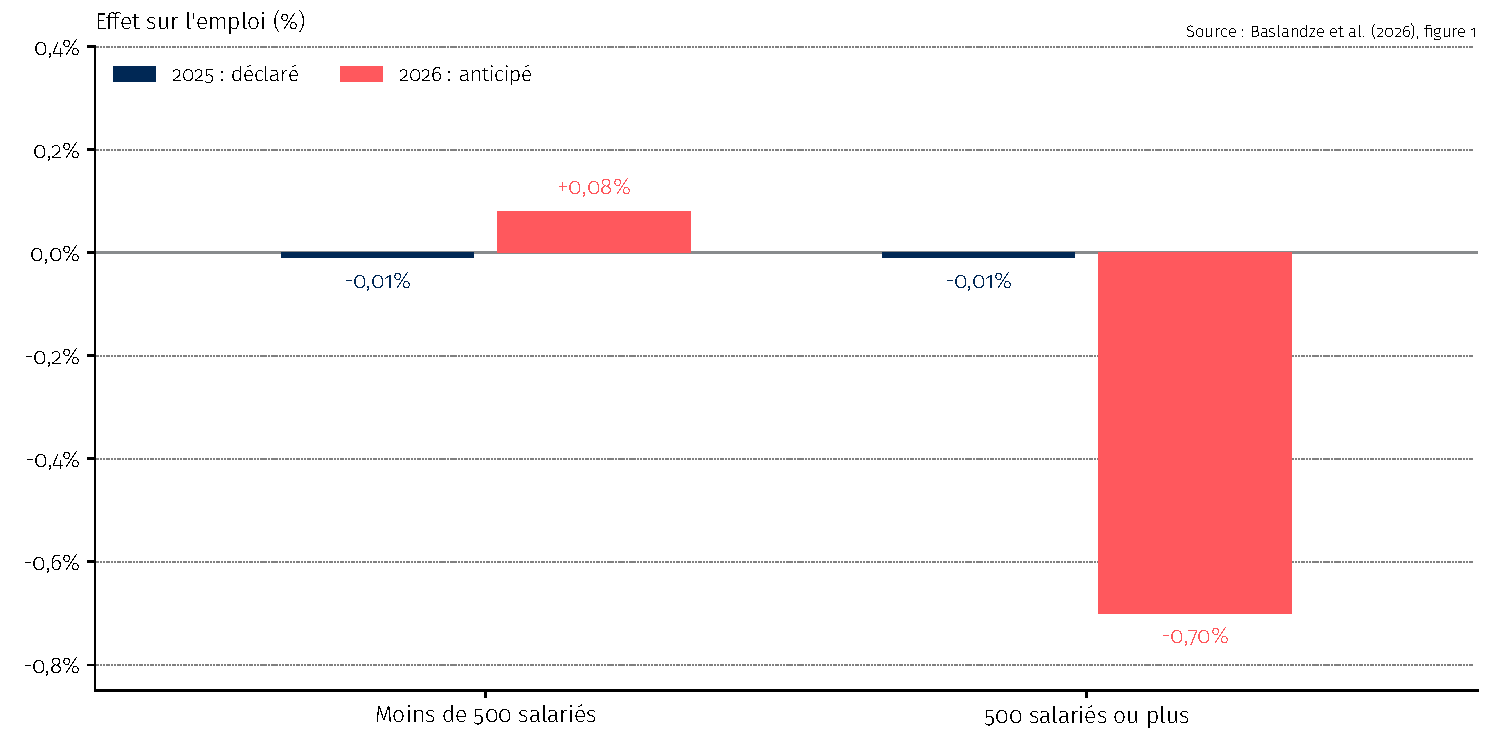
\includegraphics[width=0.95\textwidth, height=0.73\textheight, keepaspectratio]{s3_ai_cfo_employment.pdf}\par}
\end{frame}

% ============================================================================
% 40 | \begin{frame}{L'IA peut remplacer ou compléter le travail}
% Source: S3/s3.tex | \begin{frame}{L'IA peut remplacer ou compléter le travail}
% ============================================================================
\begin{frame}{L'IA peut remplacer ou compléter le travail}
   \centering
   \begin{tikzpicture}[scale=.78]
\begin{scope}
\node[font=\bfseries] at (3.7,5.9) {Travail substituable};
\draw[refline] (2.5,0) -- (2.5,2);
\node[pointlabel, below] at (2.5,0) {$L_0$};
\draw[refline] (0,2) -- (2.5,2);
\node[pointlabel, left] at (0,2) {$w_0$};
\draw[refline] (1.5625,0) -- (1.5625,1.296875);
\node[pointlabel, below] at (1.5625,0) {$L_1$};
\draw[refline] (0,1.296875) -- (1.5625,1.296875);
\node[pointlabel, left] at (0,1.296875) {$w_1$};
\draw[supply] (0,0.125) -- (6.4,4.925) node[right, curvelabel] {$L^S$};
\draw[original] (0,3.875) -- (5.166667,0) node[above right, curvelabel] {$L^D$};
\draw[curveshift, HECcoral] (0,2.46875) -- (3.291667,0) node[above right, curvelabel] {$L^{D\prime}$};
\filldraw[eqpoint=HECgray] (2.5,2) circle (3pt);
\filldraw[eqpoint=HECcoral] (1.5625,1.296875) circle (3pt);
\draw[shiftarrow, HECcoral] (3.520834,1) -- (2.270834,1);
\draw[econaxis] (0,0) -- (7.4,0) node[right] {$L$};
\draw[econaxis] (0,0) -- (0,5.6) node[above] {$w$};
\end{scope}
\begin{scope}[xshift=8.5cm]
\node[font=\bfseries] at (3.7,5.9) {Travail complémentaire};
\draw[refline] (2.5,0) -- (2.5,2);
\node[pointlabel, below] at (2.5,0) {$L_0$};
\draw[refline] (0,2) -- (2.5,2);
\node[pointlabel, left] at (0,2) {$w_0$};
\draw[refline] (3.4375,0) -- (3.4375,2.703125);
\node[pointlabel, below] at (3.4375,0) {$L_1$};
\draw[refline] (0,2.703125) -- (3.4375,2.703125);
\node[pointlabel, left] at (0,2.703125) {$w_1$};
\draw[supply] (0,0.125) -- (6.4,4.925) node[right, curvelabel] {$L^S$};
\draw[original] (0,3.875) -- (5.166667,0) node[above right, curvelabel] {$L^D$};
\draw[curveshift, HECgreen] (0,5.28125) -- (7.041667,0) node[above right, curvelabel] {$L^{D\prime}$};
\filldraw[eqpoint=HECgray] (2.5,2) circle (3pt);
\filldraw[eqpoint] (3.4375,2.703125) circle (3pt);
\draw[shiftarrow, HECgreen] (4.145834,1) -- (5.395834,1);
\draw[econaxis] (0,0) -- (7.4,0) node[right] {$L$};
\draw[econaxis] (0,0) -- (0,5.6) node[above] {$w$};
\end{scope}
\end{tikzpicture}
\end{frame}

% ============================================================================
% 41 | \begin{frame}{Le boom des centres de données aux États-Unis}
% Source: S3/s3.tex | \begin{frame}{Le boom des centres de données aux États-Unis}
% ============================================================================
\begin{frame}{Le boom des centres de données aux États-Unis}
   \begin{figure}
      \centering
      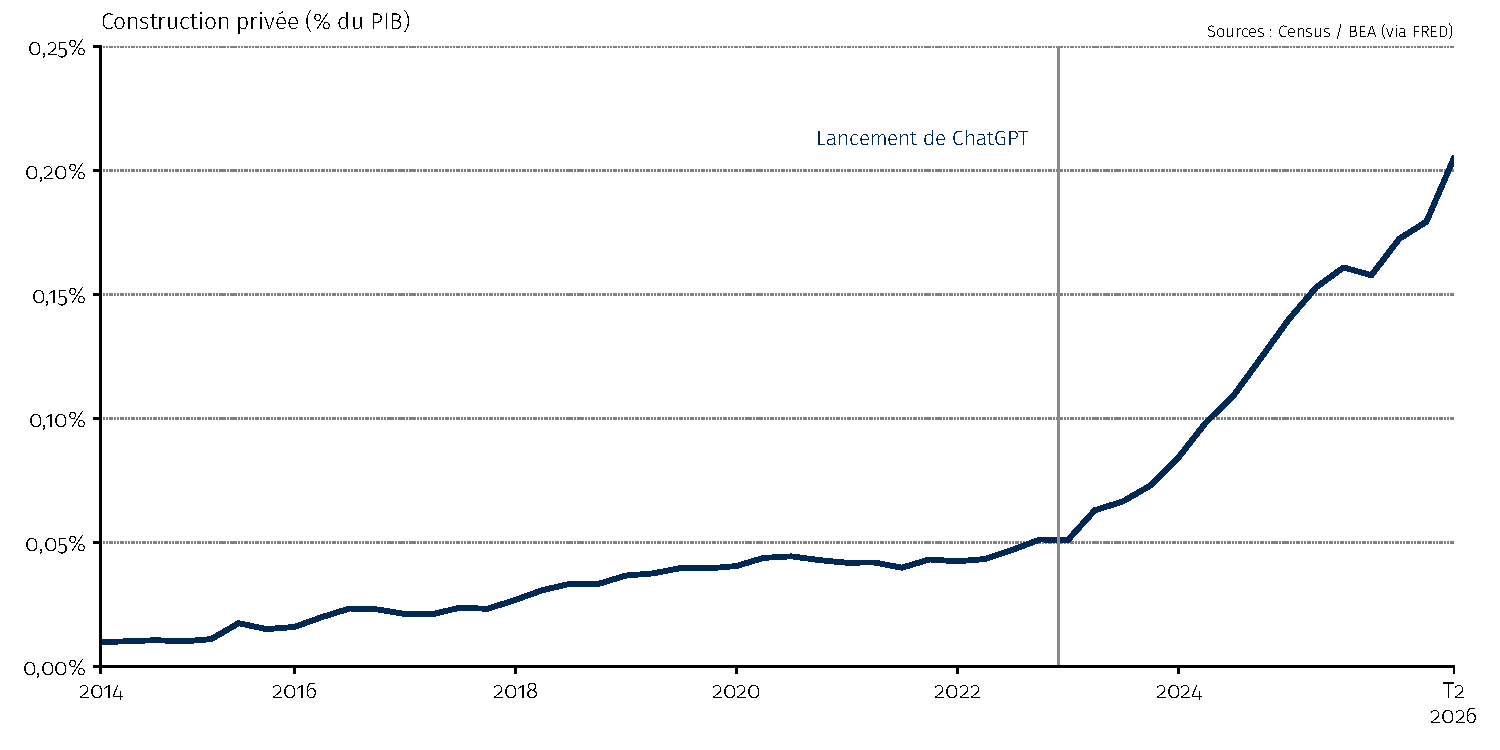
\includegraphics[width=0.95\textwidth, height=0.78\textheight, keepaspectratio]{s3_ai_datacenter_construction.pdf}
   \end{figure}
\end{frame}

% ============================================================================
% 42 | \begin{frame}{Pourquoi l'IA peut-elle relever le taux réel\,?}
% Source: S3/s3.tex | \begin{frame}{Pourquoi l'IA peut-elle relever le taux réel\,?}
% ============================================================================
\begin{frame}{Pourquoi l'IA peut-elle relever le taux réel\,?}
   \begin{columns}[c]
      \begin{column}{0.53\textwidth}
         \centering
         \begin{tikzpicture}[scale=.78]
\draw[refline] (3,0) node[below, pointlabel] {$I_0$} -- (3,2.25);
       \draw[refline] (0,2.25) node[left, pointlabel] {$r_0$} -- (3,2.25);
       \draw[refline] (4.2,0) node[below, pointlabel] {$I_1$} -- (4.2,3.15);
       \draw[refline] (0,3.15) node[left, pointlabel] {$r_1$} -- (4.2,3.15);
\draw[very thick, HECnavy] (0,0) -- (6.4,4.8) node[right, curvelabel] {$S$};
       \draw[very thick, HECcoral] (0,4.5) -- (6,0) node[above right, curvelabel] {$I$};
       \draw[curveshift, HECgreen] (0,6.3) -- (7.2,0.9) node[above right, curvelabel] {$I'$};
       \draw[shiftarrow, HECgreen] (1.733333,3.5) -- (3.333333,3.5);
\filldraw[eqpoint] (3,2.25) circle (3pt);\filldraw[eqpoint=HECgreen] (4.2,3.15) circle (3pt);
       \draw[econaxis] (0,0) -- (7.4,0) node[right] {$S, I$};
       \draw[econaxis] (0,0) -- (0,6.6) node[above] {$r$};
    \end{tikzpicture}
      \end{column}
      \begin{column}{0.43\textwidth}
         \small\RaggedRight
         \textbf{1. Plus de projets à financer}
         \par\smallskip
         À taux donné, $I$ se déplace à droite.
         \par\vspace{0.4cm}
         \textbf{2. Le taux réel augmente}
         \par\smallskip
         À épargne donnée, la hausse de $r$ équilibre le marché.
         \par\vspace{0.4cm}
         \textbf{3. D'autres projets sont évincés}
         \par\smallskip
         Certains investissements ne sont plus assez rentables.
      \end{column}
   \end{columns}
\end{frame}

% ============================================================================
% 43 | \begin{frame}[t]{Ordinateurs : la course entre prix et quantité}
% Source: S3/s3.tex | \begin{frame}[t]{Ordinateurs : la course entre prix et quantité}
% ============================================================================
\begin{frame}[t]{Ordinateurs : la course entre prix et quantité}
   \begin{columns}[T,onlytextwidth]
      \begin{column}{0.68\textwidth}
         \centering
         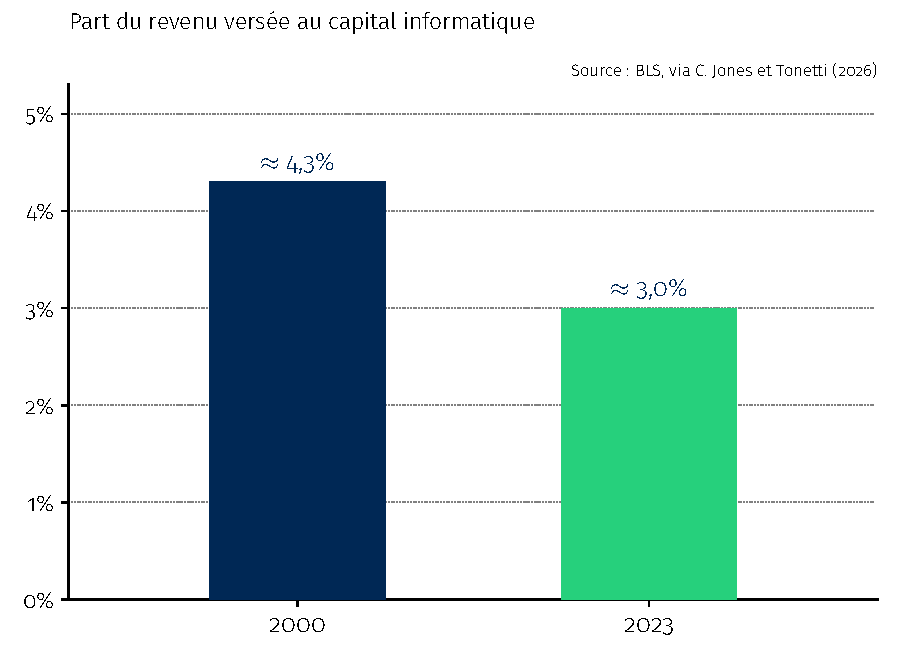
\includegraphics[width=\linewidth, height=0.57\textheight, keepaspectratio]{s3_ai_computer_income_share.pdf}
      \end{column}
      \begin{column}{0.29\textwidth}
         \small\RaggedRight
         % P is the price per unit of computing services, Q their effective volume;
         % P Q denotes payments to IT capital, not computer manufacturers' sales.
         \textbf{\textcolor{HECnavy}{Quantité : $Q \uparrow$}}
         \par\smallskip
         {\footnotesize Environ \textbf{100 millions} de fois plus de transistors par puce depuis les années 1970.\par}
         \par\vspace{0.2cm}
         \textbf{\textcolor{HECcoral}{Prix : $P \downarrow$}}
         \par\smallskip
         {\footnotesize Le progrès technique rend le calcul bien moins cher.\par}
         \par\vspace{0.2cm}
         {\footnotesize\textbf{Part du revenu}\par}
         \par\smallskip
         $\displaystyle\frac{P \times Q}{\text{revenu total}}$
      \end{column}
   \end{columns}
   \par\vspace{-0.1cm}
   \begin{keyinsight}[Le facteur rare capte la valeur]
      \RaggedRight\small
      Si le calcul abonde et complète le travail, l'humain reste le facteur rare.
   \end{keyinsight}
\end{frame}

% ============================================================================
% 44 | \begin{frame}[t]{L'IA partout, les gains de productivité où\,?}
% Source: S3/s3.tex | \begin{frame}[t]{L'IA partout, les gains de productivité où\,?}
% ============================================================================
\begin{frame}[t]{L'IA partout, les gains de productivité où\,?}
   \begin{columns}[T,onlytextwidth]
      \begin{column}{0.13\textwidth}
         {\Large\bfseries\color{HECgreen}1987}
      \end{column}
      \begin{column}{0.83\textwidth}
         \RaggedRight
         {\large\itshape\color{HECnavy}“You can see the computer age everywhere\\but in the productivity statistics.”\par}
         \par\smallskip
         {\scriptsize\href{https://www.standupeconomist.com/pdf/misc/solow-computer-productivity.pdf}{Robert Solow, \textit{New York Times Book Review}, 12 juillet 1987, p.\ 36.}\par}
      \end{column}
   \end{columns}
   \par\vspace{0.2cm}
   {\color{HECgray!30}\rule{\textwidth}{0.4pt}}
   \par\vspace{0.2cm}
   \begin{columns}[T,onlytextwidth]
      \begin{column}{0.13\textwidth}
         {\Large\bfseries\color{HECgreen}2026}
      \end{column}
      \begin{column}{0.83\textwidth}
         \small\RaggedRight
         \textbf{Le paradoxe de Solow, version IA\,?}
         \par\smallskip
         \begin{columns}[T,onlytextwidth]
            \begin{column}{0.43\textwidth}
               \RaggedRight
               {\LARGE\bfseries\color{HECnavy}$\approx 70\,\%$}\par\smallskip
               des entreprises utilisent l'IA.
            \end{column}
            \begin{column}{0.53\textwidth}
               \RaggedRight
               {\LARGE\bfseries\color{HECcoral}$> 80\,\%$}\par\smallskip
               ne déclarent aucun effet sur l'emploi ou la productivité en trois ans.
            \end{column}
         \end{columns}
         \par\vspace{0.1cm}
         {\scriptsize\href{https://www.atlantafed.org/research-and-data/publications/working-papers/2026/03/24/03-firm-data-on-ai}{Yotzov et al. (2026) : près de 6\,000 dirigeants, quatre pays ; enquête déclarative.}\par}
      \end{column}
   \end{columns}
   \par\vspace{0.1cm}
   \begin{keyinsight}[Adopter un outil ne suffit pas]
      \small\RaggedRight
      Diffuser l'outil, former les équipes et réorganiser les processus prend du temps.
   \end{keyinsight}
\end{frame}

% ============================================================================
% 45 | \begin{frame}[t]{Une infinité de chaussures droites... et alors\,?}
% Source: S3/s3.tex | \begin{frame}[t]{Une infinité de chaussures droites... et alors\,?}
% ============================================================================
\begin{frame}[t]{Une infinité de chaussures droites... et alors\,?}
   Une paire exige \textbf{une chaussure gauche et une chaussure droite}.
   \par\vspace{0.2cm}
   {\small Production par jour, à capacité inchangée pour les chaussures gauches.\par}
   \par\vspace{0.2cm}
   \renewcommand{\arraystretch}{1.4}
   \centering
   \begin{tabular}{lccc}
      \toprule
      & \textbf{Gauches} & \textbf{Droites} & \textbf{Paires} \\
      \midrule
      Avant & 100 & 100 & \textbf{100} \\
      Droites automatisées & 100 & $\infty$ & \textbf{100} \\
      \bottomrule
   \end{tabular}
   \par\vspace{0.25cm}
   \begin{keyinsight}[Les complémentarités limitent les gains]
      \small\RaggedRight
      Automatiser un maillon ne suffit pas : l'autre limite la production.
      \par\mbox{}\hfill{\scriptsize\textcolor{HECgray}{Exemple pédagogique ; \href{https://web.stanford.edu/~chadj/JonesTonetti_Automation.pdf}{maillons faibles : C. Jones et Tonetti (2026).}}}
   \end{keyinsight}
   % Perfect complements: pairs = min(left shoes,right shoes).
   % Hold left-shoe capacity fixed. Reallocating workers or expanding that
   % capacity could raise pair output; the example isolates the weak-link logic.
\end{frame}

% ============================================================================
% 46 | \begin{frame}{Baumol : les activités lentes prennent plus de place}
% Source: S3/s3.tex | \begin{frame}{Baumol : les activités lentes prennent plus de place}
% ============================================================================
\begin{frame}{Baumol : les activités lentes prennent plus de place}
   \begin{figure}
      \centering
      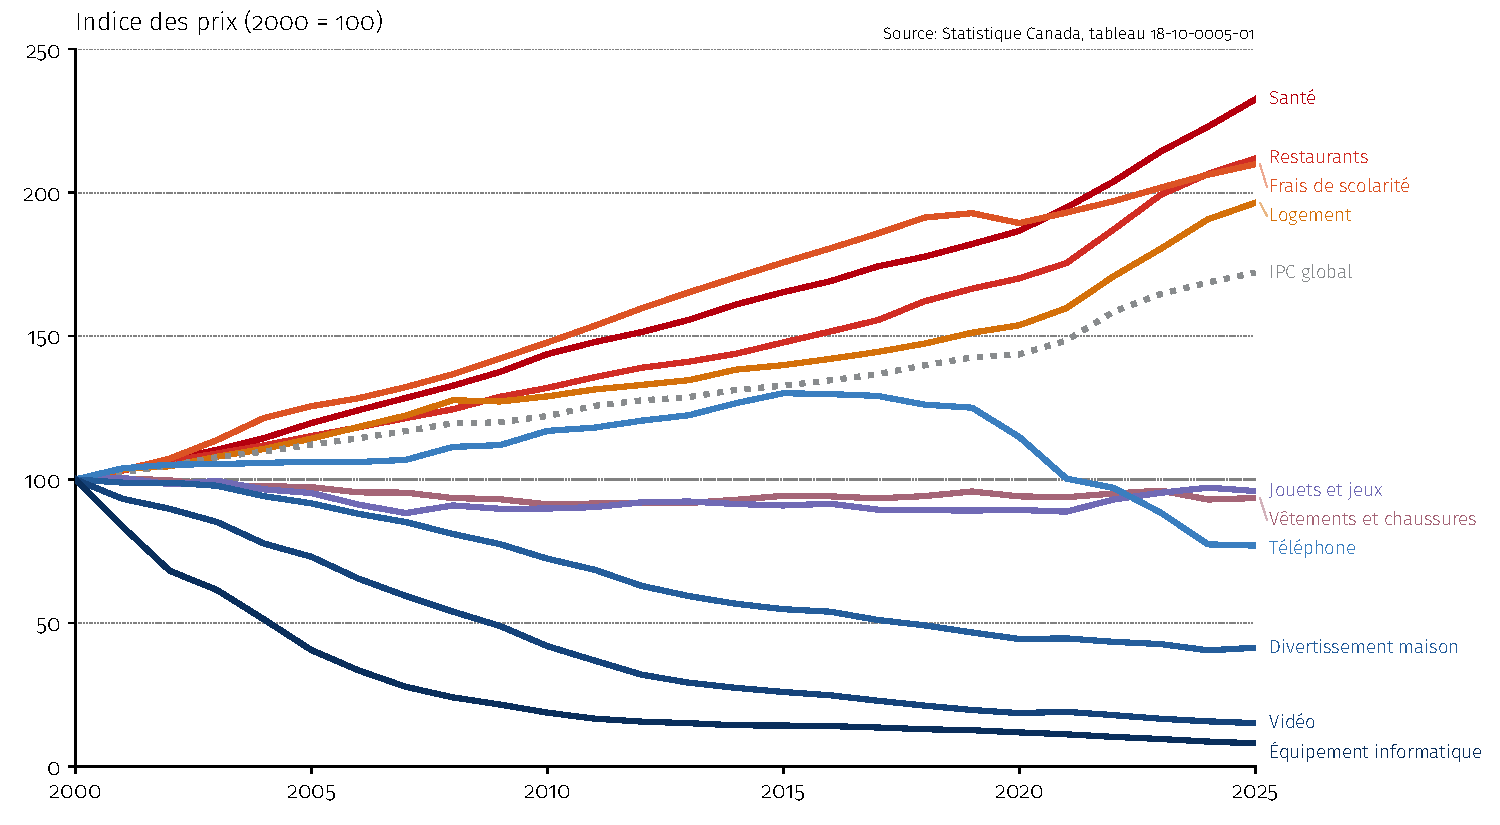
\includegraphics[width=\textwidth, height=0.80\textheight, keepaspectratio]{baumol_cost_disease_canada.pdf}
   \end{figure}
   % Oral intuition: a quartet still needs four musicians. If their wages
   % follow those elsewhere without productivity gains, its relative cost rises.
   % AI-growth link: improve essential activities whose productivity grows slowly.
   % Conceptual reference: Aghion, B. Jones and C. Jones (2019),
   % https://web.stanford.edu/~chadj/AJJ-AIandGrowth.pdf
   % The price chart illustrates relative-price differences; productivity is
   % only one of their determinants, so it does not identify a causal effect.
\end{frame}

% ============================================================================
% 47 | \begin{frame}[t]{Long terme vs.\ court terme}
% Source: S4/s4.tex | \begin{frame}[t]{Long terme vs.\ court terme}
% Adaptation: Remove references to other class sessions.
% ============================================================================
\begin{frame}[t]{Long terme vs.\ court terme}
   \begin{columns}[T]
      \begin{column}{0.48\textwidth}
         \quad \textbf{\textcolor{HECnavy}{Long terme}}
         \begin{equation*}
            \textcolor{HECgreen}{Y_{\text{POT}}} = A \cdot K^{\alpha} \cdot \textcolor{HECgreen}{L_{\text{PE}}}^{1 - \alpha}
         \end{equation*}
         \vspace{-0.5cm}
         \begin{itemize}
            \setlength\itemsep{0.15cm}
            \item $\textcolor{HECgreen}{L_{\text{PE}}}$ : niveau d'emploi de LT
            \item $\textcolor{HECgreen}{Y_{\text{POT}}}$ : PIB potentiel
            \item Marché de l'emploi en équilibre
         \end{itemize}
      \end{column}
      \begin{column}{0.48\textwidth}
         \quad \textbf{\textcolor{HECcoral}{Court terme}}
         \begin{equation*}
            \textcolor{HECcoral}{Y} = A \cdot K^{\alpha} \cdot \textcolor{HECcoral}{L}^{1 - \alpha}
         \end{equation*}
         \vspace{-0.5cm}
         \begin{itemize}
            \setlength\itemsep{0.15cm}
            \item $\textcolor{HECcoral}{L}$ : niveau d'emploi de CT
            \item $\textcolor{HECcoral}{Y}$ : PIB réel
            \item Chômage ou surchauffe possible
         \end{itemize}
      \end{column}
   \end{columns}
   \vspace{0.25cm}
   \begin{keyinsight}
      Le niveau d'emploi de CT ($\textcolor{HECcoral}{L}$) fluctue beaucoup, donc le PIB réel ($\textcolor{HECcoral}{Y}$) fluctue également autour de son potentiel ($\textcolor{HECgreen}{Y_{\text{POT}}}$). Pourquoi\,?
   \end{keyinsight}
\end{frame}

% ============================================================================
% 48 | \sectionframe{Les cycles économiques}
% Source: Shared ECON50803 title/section style
% ============================================================================
\sectionframe{Les cycles économiques}

% ============================================================================
% 49 | \begin{frame}{Que sont les cycles économiques\,?}
% Source: S4/s4.tex | \begin{frame}{Que sont les cycles économiques\,?}
% ============================================================================
\begin{frame}{Que sont les cycles économiques\,?}
   \centering
   \begin{tikzpicture}[xscale=0.9, yscale=0.9,
      peak/.style={font=\small},
      trough/.style={font=\small},
      phaseE/.style={font=\small, rotate=65, HECgreen},
      phaseR/.style={font=\small, rotate=305, HECcoral}]

      % Trend line: y = m x + b
      \def\slope{0.35}    % m
      \def\intercept{1}   % b
      \draw[refline] (0,\intercept) -- (12.8,{\slope*12.8+\intercept});

      % Cyclical component: A * sin(ω x)
      \def\amp{1.2}       % amplitude (A)
      \def\omega{90}      % ω in degrees (period = 4 units)

      % Combined path:  y(x) = trend + amp * sin(ω x)
      \draw[demand, samples=250, domain=0:13] plot (\x,{\slope*\x+\intercept + \amp*sin(\omega*\x)});

      % Identify the peaks and troughs
      \node[peak] at (1, {\slope*1 + \intercept + \amp + 0.25}) {Sommet};
      \node[trough] at (3, {\slope*3 + \intercept - \amp - 0.25}) {Creux};
      \node[peak] at (5, {\slope*5 + \intercept + \amp + 0.25}) {Sommet};
      \node[trough] at (7, {\slope*7 + \intercept - \amp - 0.25}) {Creux};
      \node[peak] at (9, {\slope*9 + \intercept + \amp + 0.25}) {Sommet};
      \node[trough] at (11, {\slope*11 + \intercept - \amp - 0.25}) {Creux};

      % Identify the phases
      \node[phaseR] at (1.75, {\slope*2 + \intercept - 0.1}) {Récession};
      \node[phaseE] at (3.75, {\slope*4+\intercept + 0.1}) {Expansion};
      \node[phaseR] at (5.75, {\slope*6 + \intercept - 0.1}) {Récession};
      \node[phaseE] at (7.75, {\slope*8+\intercept + 0.1}) {Expansion};
      \node[phaseR] at (9.75, {\slope*10 + \intercept - 0.1}) {Récession};
      \node[phaseE] at (11.75, {\slope*12+\intercept + 0.1}) {Expansion};
      % Axes (drawn last for z-order)
      \draw[econaxis] (0,0) -- (0,6) node[above]{$\ln(Y)$};
      \draw[econaxis] (0,0) -- (13,0) node[right]{$t$};
   \end{tikzpicture}
\end{frame}

% ============================================================================
% 50 | \begin{frame}{Le PIB réel et potentiel du Canada}
% Source: S4/s4.tex | \begin{frame}{Le PIB réel et potentiel du Canada}
% ============================================================================
\begin{frame}{Le PIB réel et potentiel du Canada}
   \begin{figure}
      \centering
      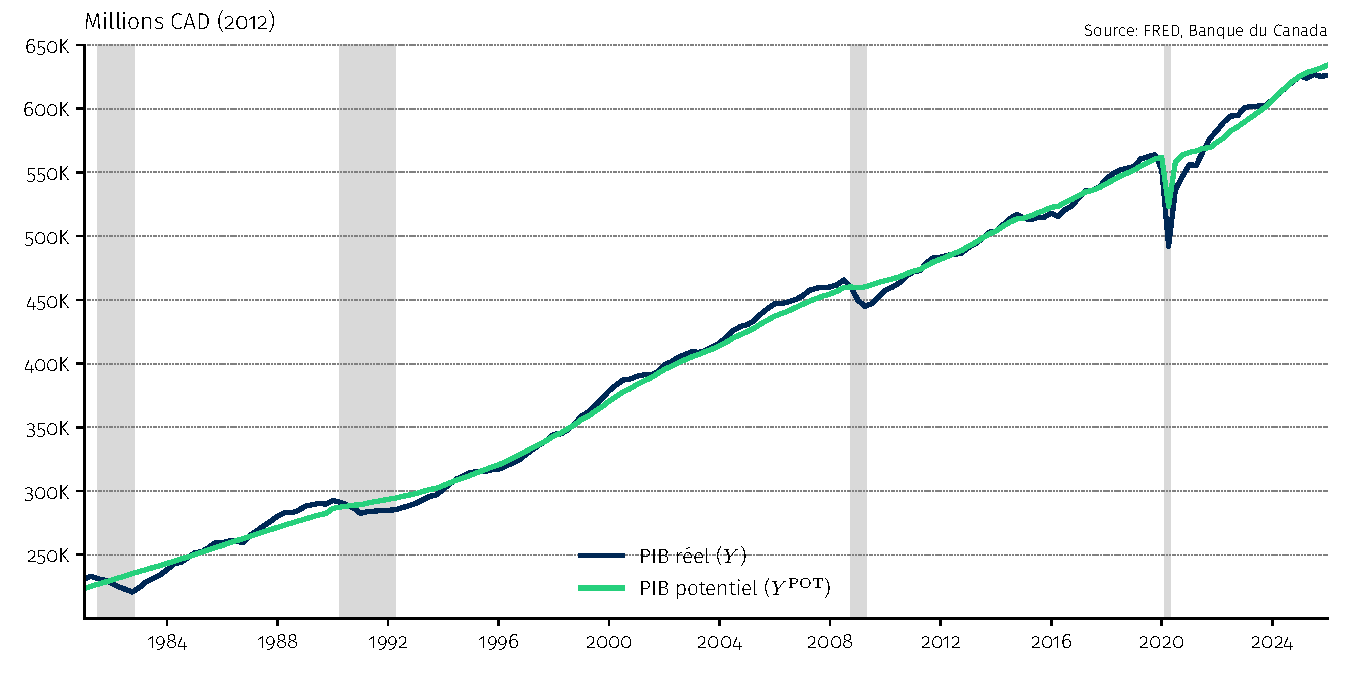
\includegraphics[width=0.95\textwidth, keepaspectratio]{canada_gdp_potential.pdf}
   \end{figure}
\end{frame}

% ============================================================================
% 51 | \begin{frame}[t]{Expansion et récession : comparer les composantes}
% Source: S1/s1.tex | \begin{frame}[t]{Expansion et récession : comparer les composantes}
% ============================================================================
\begin{frame}[t]{Expansion et récession : comparer les composantes}
   \vspace{-0.2cm}
   \begin{figure}
      \centering
      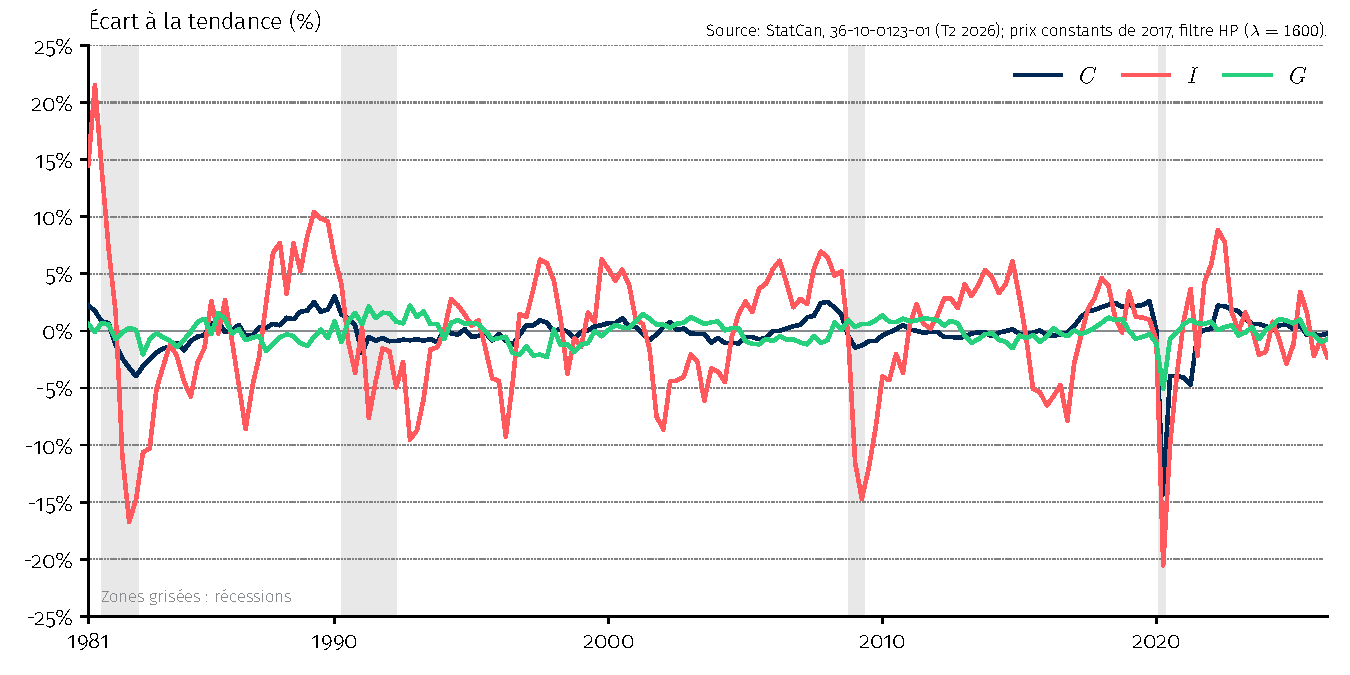
\includegraphics[width=\textwidth, height=0.79\textheight, keepaspectratio]{gdp_component_cycles.pdf}
   \end{figure}
   \vspace{-0.25cm}
   \footnotesize Au-dessus de 0 : niveau supérieur à sa \textbf{propre tendance}. $I$ inclut les stocks.
\end{frame}

% ============================================================================
% 52 | \begin{frame}[t]{Les prix et les salaires sont rigides}
% Source: S4/s4.tex | \begin{frame}[t]{Les prix et les salaires sont rigides}
% ============================================================================
\begin{frame}[t]{Les prix et les salaires sont rigides}
   \textbf{Au niveau micro :}
   \vspace{0.15cm}
   \begin{itemize}
      \setlength\itemsep{0.15cm}
      \item Durée moyenne d'un prix $\approx$ 8 mois
      \item Probabilité qu'un prix change : 11--15\,\% par mois
      \item Les salaires changent $\sim$1 fois par an
      \item Baisses de salaires très rares
      \item Les biens à forte intensité de main-d'\oe uvre ont les prix les plus rigides
   \end{itemize}
   \vspace{0.4cm}
   \textbf{Au niveau macro :}
   \vspace{0.15cm}
   \begin{itemize}
      \setlength\itemsep{0.15cm}
      \item L'inflation ne réagit pleinement aux chocs qu'après 2--3 ans
      \item Plus difficile à mesurer\ldots
   \end{itemize}
\end{frame}

% ============================================================================
% 53 | \begin{frame}[t]{Un cadre pour analyser les fluctuations}
% Source: S4/s4.tex | \begin{frame}[t]{Un cadre pour analyser les fluctuations}
% ============================================================================
\begin{frame}[t]{Un cadre pour analyser les fluctuations}
   \small
   En microéconomie, on utilise l'offre et la demande pour analyser un marché particulier (sirop d'érable, pétrole, etc.). En macro, on fait la même chose --- mais pour l'\textbf{économie dans son ensemble}.

   \vspace{0.2cm}
   \begin{itemize}
      \setlength\itemsep{0.2cm}
      \item \textbf{Demande agrégée (AD)} --- quantités demandées par les ménages ($C$), les entreprises ($I$), le gouvernement ($G$) et le reste du monde ($NX$)
      \item \textbf{Offre agrégée (AS)} --- quantités produites par l'ensemble des entreprises
   \end{itemize}

   \vspace{0.2cm}
   \begin{bizimplication}[Ce cadre permet de répondre à des questions comme\ldots]
      \footnotesize
      \vspace{-0.5cm}
      \begin{itemize}
         \setlength\itemsep{0.05cm}
         \item Pourquoi la pandémie a-t-elle causé \textit{à la fois} une récession et de l'inflation\,?
         \item Pourquoi un choc pétrolier force la BdC à choisir entre inflation et chômage\,?
      \end{itemize}
   \end{bizimplication}
\end{frame}

% ============================================================================
% 54 | \begin{frame}[t]{La demande agrégée (AD)}
% Source: S4/s4.tex | \begin{frame}[t]{La demande agrégée (AD)}
% ============================================================================
\begin{frame}[t]{La demande agrégée (AD)}
   \small
   \begin{columns}[T]
      \begin{column}{0.45\textwidth}
         \begin{defbox}[Demande agrégée]
            Relation entre niveau des prix ($P$) et niveau de dépenses ($Y$) :
            \vspace{0.15cm}

            \centering
            $Y = C + I + G + NX$
         \end{defbox}
         \vspace{0.3cm}
         \begin{keyinsight}
            Augmentation des prix $\to$ baisse de la quantité demandée.
         \end{keyinsight}
      \end{column}
      \begin{column}{0.52\textwidth}
         \centering
         \vspace{0.2cm}
         \begin{tikzpicture}[scale=1.0]
            % AD curve: y = -0.7778x + 4.389, y-int (0,4.389), x-int (5.64,0)
            \draw[demand] (0,4.389) -- (5.64,0)
               node[above right, curvelabel, text=HECnavy] {AD};
            % Points on the curve: y = 4 - (7/9)(x - 0.5)
            % At x=2: y=2.83, at x=4: y=1.28
            % Dotted reference lines
            \draw[refline] (2,0) node[below, pointlabel] {$Y_1$} -- (2,2.83);
            \draw[refline] (0,2.83) node[left, pointlabel] {$P_1$} -- (2,2.83);
            \draw[refline] (4,0) node[below, pointlabel] {$Y_2$} -- (4,1.28);
            \draw[refline] (0,1.28) node[left, pointlabel] {$P_2$} -- (4,1.28);
            % Arrow showing movement along curve
            \draw[-{Stealth[length=6pt]}, HECcoral, very thick] (2,2.83) -- (4,1.28);
            % Equilibrium dots
            \filldraw[eqpoint] (4,1.28) circle (3pt);
            \filldraw[eqpoint] (2,2.83) circle (3pt);
            % Axes (drawn last for z-order)
            \draw[econaxis] (0,0) -- (5.95,0) node[right] {$Y$};
            \draw[econaxis] (0,0) -- (0,4.7) node[above] {$P$};
         \end{tikzpicture}
      \end{column}
   \end{columns}
\end{frame}

% ============================================================================
% 55 | \begin{frame}[t]{Ce qui déplace la courbe AD}
% Source: S4/s4.tex | \begin{frame}[t]{Ce qui déplace la courbe AD}
% ============================================================================
\begin{frame}[t]{Ce qui déplace la courbe AD}
   \small
   Tout choc qui modifie les \textbf{dépenses souhaitées} à un niveau de prix donné :
   \vspace{0.5cm}
   \begin{columns}[T]
      \begin{column}{0.52\textwidth}
         \textbf{\textcolor{HECgreen}{Déplacements vers la droite}}
         \vspace{0.15cm}
         \begin{itemize}
            \setlength\itemsep{0.2cm}
            \item Hausse de la confiance ($C \uparrow$)
            \item Optimisme des entreprises ($I \uparrow$)
            \item Hausse des dépenses gouv.\ ($G \uparrow$)
            \item Boom d'exportations ($NX \uparrow$)
         \end{itemize}
         \vspace{0.2cm}
         {\footnotesize\textcolor{HECgray}{Les chocs inverses déplacent AD vers la gauche.}}
      \end{column}
      \begin{column}{0.46\textwidth}
         \centering
         \vspace{0.2cm}
         \begin{tikzpicture}[scale=0.735]
            % Original AD (dashed gray): y = -0.7346x + 4.170, y-int (0,4.170), x-int (5.68,0)
            \draw[original] (0,4.170) -- (5.68,0)
               node[above right, pointlabel] {AD};
            % Shifted AD' (green, solid): y = -0.75x + 5.325, y-int (0,5.325), x-int (7.1,0)
            \draw[curveshift, HECgreen] (0,5.325) -- (7.1,0)
               node[above right, curvelabel] {AD$'$};
            % Shift arrow: horizontal from AD to AD' at y=2.2
            \draw[shiftarrow, HECgreen] (2.92,2.2) -- (3.93,2.2);
            % Axes (drawn last for z-order)
            \draw[econaxis] (0,0) -- (7.4,0) node[right] {$Y$};
            \draw[econaxis] (0,0) -- (0,5.63) node[above] {$P$};
         \end{tikzpicture}
      \end{column}
   \end{columns}
\end{frame}

% ============================================================================
% 56 | \begin{frame}[t]{L'offre agrégée (AS)}
% Source: S4/s4.tex | \begin{frame}[t]{L'offre agrégée (AS)}
% ============================================================================
\begin{frame}[t]{L'offre agrégée (AS)}
   \small
   \begin{columns}[T]
      \begin{column}{0.45\textwidth}
         \begin{defbox}[Offre agrégée]
            Production des entreprises ($Y$) à un niveau des prix donné ($P$).
            \vspace{0.25cm}

            \textbf{Hypothèse clé :} les salaires nominaux sont rigides à court terme.
         \end{defbox}
         \vspace{0.25cm}
         \begin{keyinsight}
            À prix plus élevés $\to$ les firmes veulent produire davantage.
         \end{keyinsight}
      \end{column}
      \begin{column}{0.52\textwidth}
         \centering
         \vspace{0.2cm}
         \begin{tikzpicture}[scale=1.0]
            % AS curve: y = 0.7767x + 0.1135, y-int (0,0.1135), far end (5.2,4.16)
            \draw[supply, HECcoral] (0,0.1135) -- (5.2,4.16)
               node[right, curvelabel, text=HECcoral] {AS};
            % Dotted reference lines
            \draw[refline] (1.5,0) node[below, pointlabel] {$Y_1$} -- (1.5,1.28);
            \draw[refline] (0,1.28) node[left, pointlabel] {$P_1$} -- (1.5,1.28);
            \draw[refline] (3.5,0) node[below, pointlabel] {$Y_2$} -- (3.5,2.83);
            \draw[refline] (0,2.83) node[left, pointlabel] {$P_2$} -- (3.5,2.83);
            % Arrow showing movement along curve
            % Points on the curve: y = 0.5 + (7/9)(x - 0.5)
            % At x=1.5: y=1.28, at x=3.5: y=2.83
            \draw[-{Stealth[length=6pt]}, HECnavy, very thick] (1.5,1.28) -- (3.5,2.83);
            % Equilibrium dots
            \filldraw[eqpoint] (3.5,2.83) circle (3pt);
            \filldraw[eqpoint] (1.5,1.28) circle (3pt);
            % Axes (drawn last for z-order)
            \draw[econaxis] (0,0) -- (5.5,0) node[right] {$Y$};
            \draw[econaxis] (0,0) -- (0,4.5) node[above] {$P$};
         \end{tikzpicture}
      \end{column}
   \end{columns}
\end{frame}

% ============================================================================
% 57 | \begin{frame}[t]{Ce qui déplace la courbe AS}
% Source: S4/s4.tex | \begin{frame}[t]{Ce qui déplace la courbe AS}
% ============================================================================
\begin{frame}[t]{Ce qui déplace la courbe AS}
   \small
   Tout ce qui modifie les \textbf{coûts de production} des entreprises à prix donnés :
   \vspace{0.5cm}
   \begin{columns}[T]
      \begin{column}{0.52\textwidth}
         \textbf{\textcolor{HECgreen}{Déplacements vers la droite}}
         \vspace{0.15cm}
         \begin{itemize}
            \setlength\itemsep{0.2cm}
            \item Progrès technologique ($A \uparrow$)
            \item Baisse du prix du pétrole
            \item Baisse des salaires nominaux
            \item Amélioration des chaînes d'approvisionnement
         \end{itemize}
         \vspace{0.2cm}
         {\footnotesize\textcolor{HECgray}{Les chocs inverses déplacent AS vers la gauche.}}
      \end{column}
      \begin{column}{0.46\textwidth}
         \centering
         \vspace{0.2cm}
         \begin{tikzpicture}[scale=0.82]
            % Original AS (dashed gray): y = 0.7767x + 0.1135, y-int (0,0.1135), far end (5.26,4.2)
            \draw[original] (0,0.1135) -- (5.26,4.2)
               node[right, pointlabel] {AS};
            % Shifted AS' (green, solid): y = 0.7778x - 0.6667, x-int (0.86,0), far end (6.25,4.2)
            \draw[curveshift, HECgreen] (0.86,0) -- (6.25,4.2)
               node[right, curvelabel] {AS$'$};
            % Shift arrow: horizontal from AS to AS' at y=2.2
            % On AS: x = 0.5 + (9/7)(2.2 - 0.5) = 2.69
            % On AS': x = 1.5 + (9/7)(2.2 - 0.5) = 3.69
            \draw[shiftarrow, HECgreen] (2.87,2.2) -- (3.51,2.2);
            % Axes (drawn last for z-order)
            \draw[econaxis] (0,0) -- (6.55,0) node[right] {$Y$};
            \draw[econaxis] (0,0) -- (0,4.5) node[above] {$P$};
         \end{tikzpicture}
      \end{column}
   \end{columns}
\end{frame}

% ============================================================================
% 58 | \begin{frame}{Équilibre de court terme}
% Source: S4/s4.tex | \begin{frame}{Équilibre de court terme}
% ============================================================================
\begin{frame}{Équilibre de court terme}
   \centering
   \begin{tikzpicture}[scale=1.2]
      % AD: y = -0.6x + 4.1, y-int (0,4.1), x-int (6.833,0)
      \draw[demand] (0,4.1) -- (6.833,0) node[above right, curvelabel] {AD};
      % AS: y = 0.6x + 0.5, y-int (0,0.5), far end (6.9,4.64)
      \draw[supply, HECcoral] (0,0.5) -- (6.9,4.64) node[right, curvelabel] {AS};
      % Intersection: -0.6x+4.1 = 0.6x+0.5 => x=3.0, y=2.3
      \draw[refline] (3.0,0) node[below, pointlabel] {$Y^*$} -- (3.0,2.3);
      \draw[refline] (0,2.3) node[left, pointlabel] {$P^*$} -- (3.0,2.3);
      \filldraw[eqpoint] (3.0,2.3) circle (3pt);
      % Axes (drawn last for z-order)
      \draw[econaxis] (0,0) -- (7.2,0) node[right] {$Y$};
      \draw[econaxis] (0,0) -- (0,5.0) node[above] {$P$};
   \end{tikzpicture}
\end{frame}

% ============================================================================
% 59 | \begin{frame}[t]{Choc de demande négatif : le choc}
% Source: S4/s4.tex | \begin{frame}[t]{Choc de demande négatif : le choc}
% Adaptation: Remove a transition to an omitted long-run-adjustment slide.
% ============================================================================
\begin{frame}[t]{Choc de demande négatif : le choc}
   \vspace{0.1cm}
   \begin{columns}[T]
      \begin{column}{0.55\textwidth}
         \centering
         \begin{tikzpicture}[scale=0.875]
            % Y_POT
            \draw[potline] (3.0,0) -- (3.0,4.2)
               node[above, curvelabel, text=HECgreen] {$Y_{\text{POT}}$};
            % Dotted reference lines
            \draw[refline, HECcoral] (2.08,0) node[below, pointlabel] {$Y_1$} -- (2.08,1.75);
            \draw[refline] (0,2.3) node[left, pointlabel] {$P_0$} -- (3.0,2.3);
            \draw[refline, HECcoral] (0,1.75) node[left, pointlabel] {$P_1$} -- (2.08,1.75);
            % AS: y = 0.6x + 0.5 → y-int (0,0.5), far end (5.7,3.92)
            \draw[supply] (0,0.5) -- (5.7,3.92)
               node[right, curvelabel, text=HECnavy] {AS};
            % AD original (dashed): y = -0.6x + 4.1 → y-int (0,4.1), x-int (6.83,0)
            \draw[original] (0,4.1) -- (6.83,0)
               node[above right, curvelabel, text=HECgray] {AD};
            % AD' shifted left: y = -0.6x + 3.0 → y-int (0,3.0), x-int (5.0,0)
            \draw[curveshift, HECcoral] (0,3.0) -- (5.0,0)
               node[above right, curvelabel, text=HECcoral] {AD$'$};
            % E0: AD ∩ AS at (3.0, 2.3)
            \filldraw[eqpoint=HECgray] (3.0,2.3) circle (3pt);
            \node[pointlabel, HECgray, above right] at (3.0,2.3) {$E_0$};
            % E1: AD' ∩ AS at (2.08, 1.75)
            \filldraw[eqpoint=HECcoral] (2.08,1.75) circle (3pt);
            \node[pointlabel, HECcoral, above left] at (2.08,1.75) {$E_1$};
            % Shock arrow (AD → AD') at y=1.3: AD at x=4.67, AD' at x=2.83
            \draw[shiftarrow, HECcoral] (4.45,1.3) -- (3.2,1.3);
            \node[pointlabel, HECcoral, above] at (3.75,1.3) {Choc};
            % Axes
            \draw[econaxis] (0,0) -- (7.1,0) node[right] {$Y$};
            \draw[econaxis] (0,0) -- (0,4.5) node[above] {$P$};
         \end{tikzpicture}
      \end{column}
      \begin{column}{0.42\textwidth}
         \small
         \textbf{Court terme :}
         \vspace{0.15cm}
         \begin{enumerate}
            \setlength\itemsep{0.15cm}
            \item AD se déplace à gauche
            \item Nouvel équilibre $E_1$ : $Y$ $\downarrow$ $+$ $P$ $\downarrow$
            \item $Y_1 < Y_{\text{POT}}$ $\to$ récession
         \end{enumerate}
         \vspace{0.3cm}
         \textcolor{HECgray}{\footnotesize L'économie est en dessous de son potentiel.}
      \end{column}
   \end{columns}
\end{frame}

% ============================================================================
% 60 | \begin{frame}{Le choc d'offre : Ormuz et le pétrole}
% Source: S4/s4.tex | \begin{frame}{Le choc d'offre : Ormuz et le pétrole}
% ============================================================================
\begin{frame}{Le choc d'offre : Ormuz et le pétrole}
   \centering
   \begin{tikzpicture}[scale=1.2]
      % Y_POT (vertical)
      \draw[potline] (3.0,0) -- (3.0,4.7)
         node[above, curvelabel, text=HECgreen] {$Y_{\text{POT}}$};
      % AD original (stays in place): y = -0.6x + 4.1, y-int (0,4.1), x-int (6.833,0)
      \draw[demand] (0,4.1) -- (6.833,0)
         node[above right, pointlabel] {AD};
      % AS original (dashed gray): y = 0.6x + 0.5, y-int (0,0.5), far end (6.9,4.64)
      \draw[original] (0,0.5) -- (6.9,4.64)
         node[right, pointlabel] {AS};
      % AS' shifted a lot left: y = 0.6x + 1.5, y-int (0,1.5), far end (5.33,4.7)
      \draw[supply, HECcoral] (0,1.5) -- (5.33,4.7)
         node[right, curvelabel] {AS$'$};
      % Large AS shift arrow: from AS to AS' at y=3.2
      \draw[shiftarrow, HECcoral] (4.32,3.2) -- (3.17,3.2);
      % Reference lines
      \draw[refline] (0,2.3) node[left, pointlabel] {$P^*$} -- (3.0,2.3);
      \draw[refline] (2.17,0) node[below, pointlabel] {$Y'$} -- (2.17,2.80);
      \draw[refline] (0,2.80) node[left, pointlabel] {$P'$} -- (2.17,2.80);
      % Equilibrium dots
      \filldraw[eqfaded] (3.0,2.3) circle (3pt);
      \filldraw[eqpoint=HECcoral] (2.17,2.80) circle (3pt);
      % Axes (drawn last for z-order)
      \draw[econaxis] (0,0) -- (7.2,0) node[right] {$Y$};
      \draw[econaxis] (0,0) -- (0,5.0) node[above] {$P$};
   \end{tikzpicture}
\end{frame}

% ============================================================================
% 61 | \begin{frame}{Anatomie d'une récession}
% Source: S4/s4.tex | \begin{frame}{Anatomie d'une récession}
% Adaptation: Match the selected applications.
% ============================================================================
\begin{frame}{Anatomie d'une récession}
   Analyser une récession comme un \textbf{incendie} en quatre étapes :
   \vspace{0.3cm}
   \begin{enumerate}
      \setlength\itemsep{0.3cm}
      \item \textbf{Étincelle} --- ce qui déclenche la récession (\guillemotleft~le choc~\guillemotright)
      \item \textbf{Transmission} --- comment le choc se propage (AD, AS, ou les deux)
      \item \textbf{Carburant} --- ce qui amplifie la transmission
      \item \textbf{Pare-feu} --- la réponse politique visant à limiter les dégâts
   \end{enumerate}
   \vspace{0.3cm}
   \begin{bizimplication}[Application]
      Ce cadre aide à comprendre les effets des \textbf{tarifs} et des \textbf{chocs pétroliers}.
   \end{bizimplication}
\end{frame}

% ============================================================================
% 62 | \begin{frame}[t]{Sans représailles : un choc de demande}
% Source: S4/s4.tex | \begin{frame}[t]{Sans représailles : un choc de demande}
% Adaptation: Illustrative tariff rate; shift-arrow endpoints kept off the curves.
% ============================================================================
\begin{frame}[t]{Sans représailles : un choc de demande}
   \vspace{0.5cm}
   \begin{columns}[c]
      \begin{column}{0.55\textwidth}
         \centering
         % --- Algebraic verification ---
         % AD: P = -0.6Y + 4.1;  AS: P = 0.6Y + 0.5
         % Original eq: Y* = 3.0, P* = 2.3
         % AD': P = -0.6Y + 3.1 (tariffs shift AD left)
         % AD' ∩ AS: -0.6Y+3.1 = 0.6Y+0.5 → Y' = 2.167, P' = 1.80
         % AD' y-int (0,3.1), x-int (5.167,0)
         % Shift arrow at P=1.2: AD x=4.833, AD' x=3.167
         % ---
         \begin{tikzpicture}[scale=0.875]
            % Y_POT (vertical)
            \draw[potline] (3.0,0) -- (3.0,4.7)
               node[above, curvelabel, text=HECgreen] {$Y_{\text{POT}}$};
            % AS: y = 0.6x + 0.5, unchanged
            \draw[supply, HECcoral] (0,0.5) -- (6.9,4.64) node[right, curvelabel] {AS};
            % AD original (dashed gray): y = -0.6x + 4.1
            \draw[original] (0,4.1) -- (6.833,0)
               node[above right, pointlabel] {AD};
            % AD' shifted left: y = -0.6x + 3.1
            \draw[demand] (0,3.1) -- (5.167,0)
               node[above right, curvelabel] {AD$'$};
            % AD shift arrow at P=1.2
            \draw[shiftarrow, HECnavy] (4.63,1.2) -- (3.37,1.2);
            % Reference lines
            \draw[refline] (0,2.3) node[left, pointlabel] {$P^*$} -- (3.0,2.3);
            \draw[refline] (2.17,0) node[below, pointlabel] {$Y'$} -- (2.17,1.80);
            \draw[refline] (0,1.80) node[left, pointlabel] {$P'$} -- (2.17,1.80);
            % Equilibrium dots
            \filldraw[eqfaded] (3.0,2.3) circle (3pt);
            \filldraw[eqpoint=HECnavy] (2.17,1.80) circle (3pt);
            % Axes (drawn last for z-order)
            \draw[econaxis] (0,0) -- (7.2,0) node[right] {$Y$};
            \draw[econaxis] (0,0) -- (0,5.0) node[above] {$P$};
         \end{tikzpicture}
      \end{column}
      \begin{column}{0.42\textwidth}
         \small
         Forte exposition aux exportations vers les États-Unis.\
         \vspace{0.2cm}
         \begin{itemize}
            \setlength\itemsep{0.2cm}
            \item Exemple : tarifs de 25\,\% $\to$ $NX \downarrow$
            \item La demande pour les biens canadiens \textbf{chute}
         \end{itemize}
         \vspace{0.3cm}
         \textbf{AD se déplace vers la gauche}
         \vspace{0.2cm}

         {\footnotesize\textcolor{HECgray}{Résultat : récession ($Y \downarrow$, $P \downarrow$)}}
      \end{column}
   \end{columns}
\end{frame}

% ============================================================================
% 63 | \begin{frame}[t]{Avec représailles : le dilemme}
% Source: S4/s4.tex | \begin{frame}[t]{Avec représailles : le dilemme}
% Adaptation: Illustrative retaliation; arrow endpoints and potential-output guide cleared.
% ============================================================================
\begin{frame}[t]{Avec représailles : le dilemme}
   \vspace{0.5cm}
   \begin{columns}[c]
      \begin{column}{0.55\textwidth}
         \centering
         % --- Algebraic verification ---
         % Original: AD: P = -0.6Y + 4.1, AS: P = 0.6Y + 0.5, eq (3.0, 2.3)
         % AD': P = -0.6Y + 3.5 (moderate leftward shift — M↓ partially offsets X↓)
         %   intercept shift 0.6 → horizontal shift 1.0 unit
         % AS': P = 0.6Y + 1.9 (large leftward shift — tariffs on US inputs raise costs)
         %   intercept shift 1.4 → horizontal shift 2.333 units
         % AD' ∩ AS': -0.6Y+3.5 = 0.6Y+1.9 → 1.2Y = 1.6 → Y' = 4/3 ≈ 1.333, P' = 27/10 = 2.7
         % Stagflation: Y' < Y* (1.333 < 3.0) and P' > P* (2.7 > 2.3)
         % AD' y-int (0,3.5), x-int (5.833,0)
         % AS' y-int (0,1.9), far end (4.667,4.7)
         % AD shift arrow at P=1.0: AD x=5.167, AD' x=4.167
         % AS shift arrow at P=3.5: AS x=5.0, AS' x=2.667
         % ---
         \begin{tikzpicture}[scale=0.875]
            % Y_POT (vertical)
            \draw[potline] (3.0,0) -- (3.0,4.7)
               node[above, curvelabel, text=HECgreen] {$Y_{\text{POT}}$};
            % AD original (dashed gray): P = -0.6Y + 4.1
            \draw[original] (0,4.1) -- (6.833,0)
               node[above right, pointlabel] {AD};
            % AS original (dashed gray): P = 0.6Y + 0.5
            \draw[original] (0,0.5) -- (7.0,4.7)
               node[right, pointlabel] {AS};
            % AD' shifted left (moderate): P = -0.6Y + 3.5
            \draw[demand] (0,3.5) -- (5.833,0)
               node[above right, curvelabel] {AD$'$};
            % AS' shifted left (large — main retaliation channel): P = 0.6Y + 1.9
            \draw[supply, HECcoral] (0,1.9) -- (4.667,4.7)
               node[right, curvelabel] {AS$'$};
            % AD shift arrow at P=1.0
            \draw[shiftarrow, HECnavy] (4.97,1.0) -- (4.37,1.0);
            % AS shift arrow at P=3.5
            \draw[shiftarrow, HECcoral] (4.8,3.5) -- (3.18,3.5);
            % Reference lines
            \draw[refline] (0,2.3) node[left, pointlabel] {$P^*$} -- (3.0,2.3);
            \draw[refline] (1.333,0) node[below, pointlabel] {$Y'$} -- (1.333,2.7);
            \draw[refline] (0,2.7) node[left, pointlabel] {$P'$} -- (1.333,2.7);
            % Equilibrium dots
            \filldraw[eqfaded] (3.0,2.3) circle (3pt);
            \filldraw[eqpoint=HECcoral] (1.333,2.7) circle (3pt);
            % Axes (drawn last for z-order)
            \draw[econaxis] (0,0) -- (7.2,0) node[right] {$Y$};
            \draw[econaxis] (0,0) -- (0,5.0) node[above] {$P$};
         \end{tikzpicture}
      \end{column}
      \begin{column}{0.42\textwidth}
         \small
         Exemple de représailles : 25\,\% sur des intrants américains.\
         \vspace{0.15cm}
         \begin{itemize}
            \setlength\itemsep{0.15cm}
            \item \textbf{AS$\leftarrow$} : coûts de production $\uparrow$ (intrants importés plus chers)
            \item \textbf{AD partiellement restauré} : $M \downarrow$ $\to$ $NX$ se rétablit en partie
         \end{itemize}
         \vspace{0.2cm}
         \textbf{Double déplacement : AD$\leftarrow$ et AS$\leftarrow$}
         \vspace{0.2cm}

         {\footnotesize\textcolor{HECgray}{Résultat : stagflation ($Y \downarrow$, $P \uparrow$)}}
      \end{column}
   \end{columns}
\end{frame}

% ============================================================================
% 64 | \begin{frame}{Un scénario : pétrole cher $\to$ aubaine pour les exportateurs}
% Source: S4/s4.tex | \begin{frame}{Scénario A : Pétrole cher $\to$ aubaine pour les exportateurs}
% Adaptation: Standalone scenario title; clear arrow endpoints and labels.
% ============================================================================
\begin{frame}{Un scénario : pétrole cher $\to$ aubaine pour les exportateurs}
   \centering
   \begin{tikzpicture}[scale=1.17]
      % Y_POT (vertical)
      \draw[potline] (3.0,0) -- (3.0,4.7)
         node[above, curvelabel, text=HECgreen] {$Y_{\text{POT}}$};
      % AD original (dashed gray): y = -0.6x + 4.1, y-int (0,4.1), x-int (6.833,0)
      \draw[original] (0,4.1) -- (6.833,0)
         node[above right, pointlabel] {AD};
      % AS original (dashed gray): y = 0.6x + 0.5, y-int (0,0.5), far end (7.0,4.7)
      \draw[original] (0,0.5) -- (7.0,4.7)
         node[right, pointlabel] {AS};
      % AD' shifted slightly right: y = -0.6x + 4.5, y-int (0,4.5), x-int (7.5,0)
      \draw[demand] (0,4.5) -- (7.5,0)
         node[above right, curvelabel] {AD$'$};
      % AS' shifted a lot left: y = 0.6x + 1.5, y-int (0,1.5), far end (5.33,4.7)
      \draw[supply, HECcoral] (0,1.5) -- (5.33,4.7)
         node[right, curvelabel] {AS$'$};
      % Small AD shift arrow (rightward): from AD to AD' at y=1.5
      % AD at y=1.5: x=(4.1-1.5)/0.6=4.33; AD' at y=1.5: x=(4.5-1.5)/0.6=5.0
      \draw[shiftarrow, HECnavy] (4.46,1.5) -- (4.87,1.5);
      % Large AS shift arrow: from AS to AS' at y=3.2
      \draw[shiftarrow, HECcoral] (4.32,3.2) -- (3.17,3.2);
      % Reference lines
      \draw[refline] (0,2.3) node[left, pointlabel] {$P^*$} -- (3.0,2.3);
      \draw[refline] (2.5,0) node[below, pointlabel] {$Y'$} -- (2.5,3.0);
      \draw[refline] (0,3.0) node[left, pointlabel] {$P'$} -- (2.5,3.0);
      % Equilibrium dots
      \filldraw[eqfaded] (3.0,2.3) circle (3pt);
      \filldraw[eqpoint=HECcoral] (2.5,3.0) circle (3pt);
      % Axes (drawn last for z-order)
      \draw[econaxis] (0,0) -- (7.8,0) node[right] {$Y$};
      \draw[econaxis] (0,0) -- (0,5.0) node[above] {$P$};
   \end{tikzpicture}
   \vspace{-0.2cm}
   \par{\footnotesize\textcolor{HECcoral}{PIB $\downarrow$ modéré, prix $\uparrow\uparrow$}}
\end{frame}

% ============================================================================
% 65 | \sectionframe{Les politiques économiques}
% Source: Shared ECON50803 title/section style
% ============================================================================
\sectionframe{Les politiques économiques}

% ============================================================================
% 66 | \begin{frame}[t]{Deux institutions, deux leviers}
% Source: S5/s5.tex | \begin{frame}[t]{Deux institutions, deux leviers}
% ============================================================================
\begin{frame}[t]{Deux institutions, deux leviers}
   \vspace{0.3cm}
   \begin{columns}[T]
      \begin{column}{0.47\textwidth}
         \centering
         \textcolor{HECnavy}{\large\textbf{Politique monétaire}}\\[3pt]
         \textcolor{HECgray}{Banque centrale}\\[8pt]
         \small
         \begin{itemize}
            \setlength\itemsep{0.15cm}
            \item Taux d'intérêt directeur
            \item Décision rapide (8 annonces/an)
            \item \textbf{Indépendante} du gouvernement
            \item Agit sur AD via $C$ et $I$
         \end{itemize}
      \end{column}
      \begin{column}{0.06\textwidth}
         \centering
         \vspace{0.8cm}
         {\Large\textcolor{HECgray}{vs.\,}}
      \end{column}
      \begin{column}{0.47\textwidth}
         \centering
         \textcolor{HECgreen}{\large\textbf{Politique budgétaire}}\\[3pt]
         \textcolor{HECgray}{Gouvernement}\\[8pt]
         \small
         \begin{itemize}
            \setlength\itemsep{0.15cm}
            \item Dépenses ($G$), impôts ($T$), transferts
            \item Processus législatif (lent)
            \item Décision \textbf{politique}
            \item Agit sur AD via $G$, $C$ et $I$
         \end{itemize}
      \end{column}
   \end{columns}
\end{frame}

% ============================================================================
% 67 | \begin{frame}[t]{Un objectif clair et mesurable : cible d'inflation de 2\,\%}
% Source: S5/s5.tex | \begin{frame}[t]{Un objectif clair et mesurable : cible d'inflation de 2\,\%}
% ============================================================================
\begin{frame}[t]{Un objectif clair et mesurable : cible d'inflation de 2\,\%}
   \small
   \begin{defbox}[Entente BdC--Gouvernement]
      Cible de \textbf{2\,\%} d'inflation (depuis 1991), avec une fourchette de \textbf{1 à 3\,\%}. Renouvelée tous les 5 ans (dernière fois en 2021).
   \end{defbox}
   \vspace{0.25cm}
   \textbf{Et ailleurs dans le monde\,?}
   \vspace{0.1cm}
   \begin{itemize}
      \setlength\itemsep{0.15cm}
      \item Réserve fédérale (États-Unis) : \guillemotleft~plein emploi et stabilité des prix~\guillemotright
      \item Banque centrale européenne (zone euro) : cible d'inflation (2 \%)
      \item Banque populaire de Chine : prix, croissance, et stabilité de la devise
   \end{itemize}
\end{frame}

% ============================================================================
% 68 | \begin{frame}{Le taux directeur depuis 1996}
% Source: S5/s5.tex | \begin{frame}{Le taux directeur depuis 1996}
% ============================================================================
\begin{frame}{Le taux directeur depuis 1996}
   \begin{figure}
      \centering
      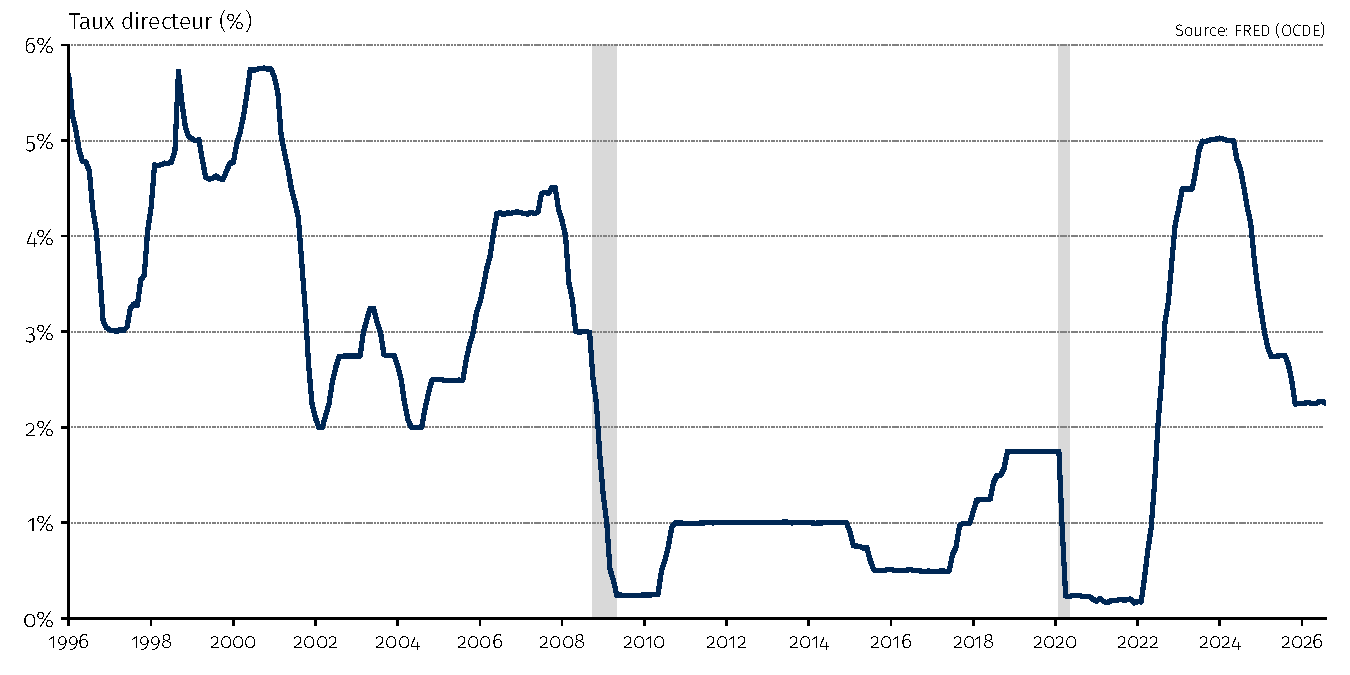
\includegraphics[width=0.95\textwidth, height=0.78\textheight, keepaspectratio]{overnight_rate_ca.pdf}
   \end{figure}
\end{frame}

% ============================================================================
% 69 | \begin{frame}{Le mécanisme de transmission}
% Source: S5/s5.tex | \begin{frame}{Le mécanisme de transmission}
% ============================================================================
\begin{frame}{Le mécanisme de transmission}
   \centering
   \vspace{0.1cm}
   \begin{tikzpicture}[
      box/.style={rectangle, rounded corners=8pt, draw=HECnavy, line width=0.8pt,
                  fill=HEClightgray, minimum width=2.8cm, minimum height=1cm,
                  align=center, font=\small, inner sep=5pt}]
      % 4 nodes on an ellipse (wider horizontally)
      \node[box] (td)  at (0, 2.6)  {Taux directeur};
      \node[box] (tm)  at (3.8, 0)  {Taux du marché};
      \node[box] (dep) at (0,-2.6)  {$C$, $I$, $NX$};
      \node[box] (pib) at (-3.8, 0) {PIB $+$ inflation};
      % Curved arrows (clockwise, bend left = outward curvature)
      \draw[flowarrow] (td) to[bend left=25]
         node[above right=-2pt, pointlabel, text=HECnavy] {Prêts, obligations} (tm);
      \draw[flowarrow] (tm) to[bend left=25]
         node[right=1pt, pointlabel, text=HECnavy] {Coût d'emprunt} (dep);
      \draw[flowarrow] (dep) to[bend left=25]
         node[below left=-2pt, pointlabel, text=HECnavy] {Demande agrégée} (pib);
      % Feedback arrow (dashed, closes the loop)
      \draw[flowarrow, HECgray, dashed] (pib) to[bend left=25]
         node[left=1pt, pointlabel, text=HECgray] {Rétroaction} (td);
      % Delay annotation
      \node[font=\scriptsize, HECcoral, align=center] at (0,0) {Délai total : \textbf{6 à 8 trimestres}};
   \end{tikzpicture}
\end{frame}

% ============================================================================
% 70 | \begin{frame}[t]{Politique expansionniste : la réponse de la BdC}
% Source: S5/s5.tex | \begin{frame}[t]{Politique expansionniste : la réponse de la BdC}
% ============================================================================
\begin{frame}[t]{Politique expansionniste : la réponse de la BdC}
   \vspace{0.1cm}
   \begin{columns}[T]
      \begin{column}{0.55\textwidth}
         \centering
         \begin{tikzpicture}[scale=0.875]
            % Y_POT
            \draw[potline] (3.0,0) -- (3.0,4.2)
               node[above, curvelabel, text=HECgreen] {$Y_{\text{POT}}$};
            % Dotted reference lines
            \draw[refline] (2.08,0) node[below, pointlabel] {$Y_1$} -- (2.08,1.75);
            \draw[refline, HECnavy] (0,2.3) node[left, pointlabel] {$P_2$} -- (3.0,2.3);
            \draw[refline] (0,1.75) node[left, pointlabel] {$P_1$} -- (2.08,1.75);
            % AS: y = 0.6x + 0.5 → y-int (0,0.5), far end (6.8,4.58)
            \draw[supply] (0,0.5) -- (6.8,4.58)
               node[right, curvelabel, text=HECnavy] {AS};
            % AD' (recession, now dashed): y = -0.6x + 3.0 → y-int (0,3.0), x-int (5.0,0)
            \draw[original] (0,3.0) -- (5.0,0)
               node[above right, curvelabel, text=HECgray] {AD$'$};
            % AD'' (after policy, back to original): y = -0.6x + 4.1 → y-int (0,4.1), x-int (6.83,0)
            \draw[demand] (0,4.1) -- (6.83,0)
               node[above right, curvelabel, text=HECnavy] {AD$''$};
            % E1: AD' ∩ AS at (2.08, 1.75)
            \filldraw[eqpoint=HECgray] (2.08,1.75) circle (3pt);
            \node[pointlabel, HECgray, above left] at (2.08,1.75) {$E_1$};
            % E2: AD'' ∩ AS at (3.0, 2.3) — back at potential
            \filldraw[eqpoint=HECnavy] (3.0,2.3) circle (3pt);
            \node[pointlabel, HECnavy, above right] at (3.0,2.3) {$E_2$};
            % Policy arrow
            \draw[shiftarrow, HECnavy] (3.1,1.3) -- (4.45,1.3);
            \node[pointlabel, HECnavy, above] at (3.5,1.3) {$\downarrow$ taux};
            % Axes
            \draw[econaxis] (0,0) -- (7.1,0) node[right] {$Y$};
            \draw[econaxis] (0,0) -- (0,4.9) node[above] {$P$};
         \end{tikzpicture}
      \end{column}
      \begin{column}{0.42\textwidth}
         \small
         \textbf{Réponse de politique monétaire :}
         \vspace{0.15cm}
         \begin{enumerate}
            \setlength\itemsep{0.1cm}
            \item BdC $\downarrow$ taux directeur
            \item Taux du marché $\downarrow$
            \item $C\uparrow$, $I\uparrow$, $NX\uparrow$ $\to$ AD$''$ à droite
            \item Retour à $Y_{\text{POT}}$ en $E_2$
         \end{enumerate}
         \vspace{0.2cm}
         \begin{keyinsight}[Avantage]
            Retour à $Y_{\text{POT}}$ \textbf{plus rapide} que l'ajustement par les salaires.
         \end{keyinsight}
      \end{column}
   \end{columns}
\end{frame}

% ============================================================================
% 71 | \begin{frame}[t]{Les délais de transmission}
% Source: S5/s5.tex | \begin{frame}[t]{Les délais de transmission}
% ============================================================================
\begin{frame}[t]{Les délais de transmission}
   \small
   \vspace{0.2cm}
   \textbf{Consensus :} 6 à 8 trimestres entre la décision et l'effet maximal sur l'inflation.
   \vspace{0.2cm}
   \begin{itemize}
      \setlength\itemsep{0.2cm}
      \item La BdC doit donc agir en fonction de ses \textbf{prévisions}, pas de la situation actuelle
      \item Les prévisions sont \textbf{imparfaites} --- c'est loin d'être une science exacte
      \item Métaphore : \guillemotleft~conduire en regardant dans le rétroviseur~\guillemotright
   \end{itemize}
   \vspace{0.2cm}
   \begin{keyinsight}
      C'est pour cette raison que les banques centrales répètent que leurs décisions sont \guillemotleft~\textit{forward-looking}~\guillemotright\ et dépendent des \guillemotleft~données à venir~\guillemotright.
   \end{keyinsight}
\end{frame}

% ============================================================================
% 72 | \begin{frame}[t]{Le dilemme des chocs d'offre}
% Source: S5/s5.tex | \begin{frame}[t]{Le dilemme des chocs d'offre}
% Adaptation: P is a price level, consistent with the AD-AS axes.
% ============================================================================
\begin{frame}[t]{Le dilemme des chocs d'offre}
   \small
   \vspace{0.1cm}
   \begin{columns}[T]
      \begin{column}{0.55\textwidth}
         \centering
         \begin{tikzpicture}[scale=0.9]
            % Y_POT
            \draw[potline] (3.0,0) -- (3.0,4.2)
               node[above, curvelabel, text=HECgreen] {$Y_{\text{POT}}$};
            % Dotted reference lines
            \draw[refline, HECcoral] (2.25,0) node[below, pointlabel] {$Y_1$} -- (2.25,2.75);
            \draw[refline] (0,2.3) node[left, pointlabel] {$P_0$} -- (3.0,2.3);
            \draw[refline, HECcoral] (0,2.75) node[left, pointlabel] {$P_1$} -- (2.25,2.75);
            % AS original (dashed): y = 0.6x + 0.5 → y-int (0,0.5), far end (6.8,4.58)
            \draw[original] (0,0.5) -- (6.8,4.58)
               node[right, curvelabel, text=HECgray] {AS};
            % AD: y = -0.6x + 4.1 → y-int (0,4.1), x-int (6.83,0)
            \draw[demand] (0,4.1) -- (6.83,0)
               node[above right, curvelabel, text=HECnavy] {AD};
            % AS' shifted left: y = 0.6x + 1.4 → y-int (0,1.4), far end (5.33,4.6)
            \draw[curveshift, HECcoral] (0,1.4) -- (5.33,4.6)
               node[right, curvelabel, text=HECcoral] {AS$'$};
            % E0: AS ∩ AD at (3.0, 2.3)
            \filldraw[eqpoint=HECgray] (3.0,2.3) circle (3pt);
            \node[pointlabel, HECgray, below left] at (3.0,2.3) {$E_0$};
            % E1: AS' ∩ AD at (2.25, 2.75)
            \filldraw[eqpoint=HECcoral] (2.25,2.75) circle (3pt);
            \node[pointlabel, HECcoral, above left] at (2.25,2.75) {$E_1$};
            % Shock arrow (AS → AS') — horizontal between the two AS curves
            \draw[shiftarrow, HECcoral] (4.8,3.5) -- (3.7,3.5);
            \node[pointlabel, HECcoral, above] at (4.6,3.5) {Choc};
            % Axes
            \draw[econaxis] (0,0) -- (7.1,0) node[right] {$Y$};
            \draw[econaxis] (0,0) -- (0,4.9) node[above] {$P$};
         \end{tikzpicture}
      \end{column}
      \begin{column}{0.42\textwidth}
         \small
         \textbf{Le problème :}
         \vspace{0.1cm}
         \begin{enumerate}
            \setlength\itemsep{0.1cm}
            \item AS se déplace à gauche
            \item $Y$ $\downarrow$ \textbf{et} $P$ $\uparrow$ simultanément
            \item La banque centrale ne peut pas corriger les deux à la fois
         \end{enumerate}
         \vspace{0.15cm}
         \footnotesize
         \renewcommand{\arraystretch}{1.15}
         \begin{tabular}{@{}lcc@{}}
            & PIB ($Y$) & prix ($P$) \\[2pt]
            \hline\\[-6pt]
            $\uparrow$ taux directeur & $\downarrow$ & $\downarrow$ \\[2pt]
            $\downarrow$ taux directeur & $\uparrow$ & $\uparrow$ \\[2pt]
         \end{tabular}
         \vspace{0.15cm}

         \textcolor{HECgray}{\scriptsize Avec un choc de demande, la BdC peut stabiliser $Y$ et $P$ en même temps. Avec un choc d'offre, elle doit \textbf{choisir}.}
      \end{column}
   \end{columns}
\end{frame}

% ============================================================================
% 73 | \begin{frame}[t]{L'autre levier : le gouvernement}
% Source: S5/s5.tex | \begin{frame}[t]{L'autre levier : le gouvernement}
% Adaptation: Keep the Canadian G/I convention and the transfer channel consistent.
% ============================================================================
\begin{frame}[t]{L'autre levier : le gouvernement}
   \small
   \textbf{Trois canaux pour stimuler la demande agrégée :}
   \vspace{0.2cm}
   \begin{enumerate}
      \setlength\itemsep{0.2cm}
      \item \textbf{Dépenses publiques ($G \uparrow$)} --- effet direct sur le PIB (services publics, défense, santé)
      \item \textbf{Transferts aux ménages} --- effet indirect via $C$ (chèques, assurance-emploi)
      \item \textbf{Baisses d'impôts ($T \downarrow$)} --- effet indirect via $C$ et $I$ (revenu disponible $\uparrow$)
   \end{enumerate}
   \vspace{0.2cm}
   Certains de ces canaux agissent comme des \textbf{stabilisateurs automatiques} : l'assurance-emploi et l'impôt progressif ajustent $T$ et les transferts \textbf{sans décision politique}.
   \vspace{0.15cm}
   \begin{keyinsight}[Différence fondamentale]
      $G$ entre \textbf{directement} dans le PIB ($Y = C + I + G + NX$). Les transferts soutiennent la demande si les ménages \textbf{dépensent} l'argent reçu.
   \end{keyinsight}
\end{frame}

% ============================================================================
% 74 | \begin{frame}[t]{Déficit vs dette : flux vs stock}
% Source: S5/s5.tex | \begin{frame}[t]{Déficit vs dette : flux vs stock}
% Adaptation: Qualify the simplified stock-flow identity.
% ============================================================================
\begin{frame}[t]{Déficit vs dette : flux vs stock}
   \small
   \vspace{-0.25cm}
   \begin{columns}[T]
      \begin{column}{0.47\textwidth}
         \begin{defbox}[Déficit budgétaire]
            \footnotesize
            Recettes $<$ Dépenses en une année.\\[4pt]
            Le déficit est un \textbf{flux} : il mesure le déséquilibre \textit{pendant} une période.
         \end{defbox}
      \end{column}
      \begin{column}{0.47\textwidth}
         \begin{defbox}[Dette publique]
            \footnotesize
            Accumulation des déficits passés et des ajustements.\\[4pt]
            La dette est un \textbf{stock} : elle mesure le total \textit{à un moment donné}.
         \end{defbox}
      \end{column}
   \end{columns}
   \vspace{0.3cm}
   \centering
   Relation simplifiée, hors ajustements comptables\,:\\[4pt]
   {\large $\text{Dette}_{t} = \text{Dette}_{t-1} + \text{Déficit}_{t}$}
   \vspace{0.15cm}
   \begin{keyinsight}
      On mesure souvent la dette en \textbf{\,\% du PIB} pour la comparer entre pays et dans le temps. Un pays qui croît rapidement peut absorber plus de dette.
   \end{keyinsight}
\end{frame}

% ============================================================================
% 75 | \begin{frame}[t]{Comparaison : politique monétaire vs.\ budgétaire}
% Source: S5/s5.tex | \begin{frame}[t]{Comparaison : politique monétaire vs.\ budgétaire}
% ============================================================================
\begin{frame}[t]{Comparaison : politique monétaire vs.\ budgétaire}
   \small
   \vfill
   \renewcommand{\arraystretch}{1.75}
   \centering
   \begin{tabularx}{\textwidth}{>{\bfseries\small}l >{\small}X >{\small\raggedright\arraybackslash}p{0.42\textwidth}}
      \toprule
      & \textbf{Politique monétaire} & \textbf{Politique budgétaire} \\
      \midrule
      Décideur & Banque centrale & Gouvernement \\
      Rapidité & Rapide (8 annonces/an) & Lente (processus législatif) \\
      Indépendance & Oui & Non (politique) \\
      Canal & Taux $\to$ $C$, $I$, $NX$ & $G$ direct + $C, I$ via transferts/impôts \\
      Précision & Faible (effets diffus) & Peut cibler des secteurs \\
      Limite & Délai, incert., borne zéro & \textcolor{HECcoral}{\textbf{Endettement}} \\
      \bottomrule
   \end{tabularx}
   \vfill
\end{frame}

% ============================================================================
% 76 | \begin{frame}{Que faire face à une récession\,?}
% Source: S4/s4.tex | \begin{frame}{Que faire face à une récession\,?}
% Adaptation: Remove a reference to another class session.
% ============================================================================
\begin{frame}{Que faire face à une récession\,?}
   \vspace{0.3cm}
   \textbf{Analyse en quatre étapes :}
   \vspace{0.3cm}
   \begin{enumerate}
      \setlength\itemsep{0.3cm}
      \item {\color{gray!50}Étincelle --- ce qui déclenche la récession}
      \item {\color{gray!50}Transmission --- comment le choc se propage}
      \item {\color{gray!50}Carburant --- ce qui amplifie la transmission}
      \item \textbf{\textcolor{HECnavy}{Pare-feu --- réponse politique pour limiter les dégâts}}
   \end{enumerate}
   \vspace{0.3cm}
   \begin{keyinsight}
      L'économie peut se corriger seule, mais \textbf{attendre coûte cher} (chômage, faillites). C'est le fondement de la politique contracyclique.
   \end{keyinsight}
\end{frame}

% ============================================================================
% 77 | \begin{frame}[t]{Ce que cela change pour votre organisation}
% Source: Programme-specific closing synthesis
% ============================================================================
\begin{frame}[t]{Ce que cela change pour votre organisation}
   \RaggedRight

\small\renewcommand{\arraystretch}{1.6}
\begin{tabularx}{\textwidth}{@{}>{\bfseries}lJ@{}}
\toprule
Canal & Hypothèses à suivre\\
\midrule
Clients & Volumes, prix de vente, pouvoir d'achat et marchés d'exportation\\
Fournisseurs & Énergie, transport, intrants et délais d'approvisionnement\\
Employés & Disponibilité, compétences, salaires et complémentarités technologiques\\
Financement & Coût du crédit, renouvellements et rentabilité des projets\\
\bottomrule
\end{tabularx}

\par\vspace{0.15cm}
\begin{keyinsight}[Raisonner en scénarios]\small\RaggedRight
Relier les signaux macroéconomiques à votre exposition, puis réviser les hypothèses lorsque les données changent.
\end{keyinsight}
\end{frame}

% ============================================================================
% 78 | \begin{frame}[t]{Les grands thèmes du cours}
% Source: Programme-specific closing synthesis
% ============================================================================
\begin{frame}[t]{Les grands thèmes du cours}
\RaggedRight\small
\renewcommand{\arraystretch}{1.35}
\begin{tabularx}{\textwidth}{@{}>{\bfseries\raggedright\arraybackslash}p{0.26\textwidth}J@{}}
\toprule
\textbf{Thème} & \textbf{Idée à retenir}\\
\midrule
\textcolor{HECnavy!40}{Mesurer l'économie} & \textcolor{HECnavy!40}{Distinguer production, prix, population et emploi.}\\
\textcolor{HECnavy!40}{Croissance} & \textcolor{HECnavy!40}{Le capital aide ; la productivité soutient le niveau de vie.}\\
\textcolor{HECnavy!40}{Travail et capital} & \textcolor{HECnavy!40}{Salaires et financement reflètent les besoins et les ressources disponibles.}\\
\textcolor{HECnavy!40}{Cycles} & \textcolor{HECnavy!40}{Distinguer les chocs de demande et d'offre.}\\
\textcolor{HECnavy!40}{Politiques} & \textcolor{HECnavy!40}{Choisir les instruments selon le diagnostic et leurs limites.}\\
\bottomrule
\end{tabularx}
\end{frame}

\end{document}
